\documentclass{book}
\usepackage{commeunjeustyle}
\begin{document}


\chapter*{Application linéaire}


\begin{Texte}
Comme souvent en mathématiques, ce sont plus les transformations qui sont intéressantes et pertinentes que les objets eux-mêmes.\\
Une application linéaire est un cas particulier de transformation.  Dans le langage courant, un phénomène est dit linéaire si les
effets sont proportionnels aux causes. \\
Plus précisément, un phénomène peut être décrit par une transformation$x \mapsto f (x)$, où $x$ représente la ou les causes (par exemple une différence de
potentiel) et $f(x)$ un effet auquel on s'intéresse (par exemple l'intensité
d'un courant électrique). On dit que le phénomène est linéaire quand  l'effet est proportionnel à la cause (exemple : l'intensité de courant est
proportionnel à la différence de potentiel, en d'autres termes, si on double
la différence de potentiel, on double l'intensité du courant résultant, si on somme de deux différence de potentiel, on somme l'intensité du courant résultant).
Beaucoup de phénomènes en sciences ne sont pas linéaires. Dans de tels
cas, de "petites causes" peuvent avoir de "grands effets".\\
D'un point de vue mathématiques, une
transformation préservant la structure d'espace vectoriel est une application linéaire.  Les matrices sont des tableaux de nombres qui servent à interpréter en termes calculatoires et donc opérationnels les applications linéaires dont les espaces vectoriels sont de dimensions finies.\\ 
\begin{Exemple}[Système d'équations linéaires]
La somme des tailles d'un fils et du père est de 2,5 mètres. La différence de tailles  est de 0.5 mètres.
Quel est la taille du fils ? \\
Comme vu au chapitre précédent, la première étape est la modélisation avec un système d'équations linéaires.\\
Soit la variable $x$ représentant la taille du fils et la variable $y$ représentant la taille du père.\\
Le couple $(x,y)$ vérifie le système suivant  :
$$(S)\quad \begin{cases}
x+y&=2,5\\
-x+y&=0,5
\end{cases}
$$
L'idée est de considérer les membres de gauche des équations comme l'image d'une fonction :
\begin{center}
$
\begin{cases}
{\color{red}x}+{\color{green}y}&={\color{blue}2,5}\\
{\color{red}-x}+{\color{green}y}&={\color{blue}0,5}
\end{cases}
\Leftrightarrow\quad \begin{pmatrix}
 {\color{red}x} +{\color{green}y}   \\
 {\color{red}-x} +{\color{green}y}   \\
\end{pmatrix} =\begin{pmatrix}
 {\color{blue}2,5}   \\
 {\color{blue}0,5}  \\
\end{pmatrix}
\Leftrightarrow\quad
u(\begin{pmatrix}
 \color{red}x     \\ {\color{green}y}   \\
\end{pmatrix})
	 = \begin{pmatrix}
 {\color{blue}2,5}   \\
 {\color{blue}0,5}  \\
\end{pmatrix}$\\
\begin{tikzpicture}[general,scale=1]
\draw [->, epais] (0,0)node[left]{avec $\quad \begin{pmatrix}
 {\color{red}x}    \\
{\color{green}y}   \\
\end{pmatrix}$} -- (1,0);
\draw [-, epais] (1,-1)--(2.5,-1)--(2.5,1)--(1,1)--(1,-1);
\draw(1.75,0) node{$u$};
\draw [->, epais] (2.5,0) -- (3.5,0)node[right]{$\begin{pmatrix}
 {\color{red}x} + {\color{green}y}    \\
 {\color{red}-x}+  {\color{green}y}   \\
\end{pmatrix}$};
\end{tikzpicture} 
\end{center}
Les solutions du système sont l'ensemble des antécédents $\begin{pmatrix}
 {\color{blue}2,5}   \\
 {\color{blue}0,5}  \\
\end{pmatrix}$ de la fonction à deux variables $\Fonction{u}{\R^2}{\R^2}{\begin{pmatrix}
  {\color{red}x}    \\
 {\color{green}y}   \\
\end{pmatrix}}{\begin{pmatrix}
  {\color{red}x} +{\color{green}y}   \\
  {\color{red}-x} +{\color{green}y}   \\
\end{pmatrix}}$.\\
L'étude générale des fonctions à plusieurs variables est compliquée et est fait dans un cours d'analyse.  
Cependant, comme la fonction $u$ est linéaire :
 $$u(\begin{pmatrix}
 {x}    \\
{y}   \\
\end{pmatrix}+\begin{pmatrix}
 {x'}    \\
{y'}   \\
\end{pmatrix})=u(\begin{pmatrix}
 {x}    \\
{y}   \\
\end{pmatrix})+u(\begin{pmatrix}
 {x'}    \\
{y'}   \\
\end{pmatrix}) \quad\text{ et }\quad u(\lambda \begin{pmatrix}
 {x}    \\
{y}   \\
\end{pmatrix})=\lambda u(\begin{pmatrix}
 {x}    \\
{y}   \\
\end{pmatrix})$$
on aura des outils pour démontrer que $u$ est un isomorphisme. Ainsi il existe une unique vecteur antécédent au vecteur $\begin{pmatrix}
 {\color{blue}2,5}   \\
 {\color{blue}0,5}  \\
\end{pmatrix}$. Le système admet une unique solution.
\end{Exemple}
Notations :
\begin{itemize}
\item $\K $ désigne le corps $\R $ ou $\C $
\item $E$ et $F$ deux $\K$-espaces vectoriels
\end{itemize}
\end{Texte}


\section{Applications linéaires}

\subsection{Définition}



\begin{Definition}[Application linéaire]
Soit $E$ et $F$ deux $\K $-espaces vectoriels.\\
Une application $u:E\to F$ est dite \defi{linéaire}, si  elle préserve la structure d'espace vectoriel, c'est à dire si :
\begin{itemize}
\item
  \defi{additivité} : $\forall   \Vect{x},\Vect{y}\in  E:\quad u(\Vect{x}+\Vect{y}) = u(\Vect{x}) + u(\Vect{y})$;
\item
  \defi{homogénéité} : $\forall   \lambda \in  \K,\forall   \Vect{x}\in  E:\quad u(\lambda \Vect{x}) = \lambda u(\Vect{x})$.
\end{itemize}
\end{Definition}
\begin{Exemple} 
\begin{itemize}
\item homothétie vectorielle de rapport $\lambda$ : $\Fonction{\Phi _0}{E}{E}{\Vect{x}}{\lambda\vec{x}}$ 
\item Équation d'un plan : $\Fonction{\Phi _1}{\mathbb {R}^3 }{\mathbb {R}}{(x,y,z)}{x+y+3z}$,
\item Intégration :$\Fonction{\Phi _2}{\mathcal{C}([0,1]),  \mathbb {R} }{\mathbb {R}}{f}{\int_0^1 f(x)dx}$,
\item Dérivé de polynôme de degré au plus $n$ : $\Fonction{\Phi _3}{\mathbb {R}_n[X] }{\mathbb {R}_n[X]}{P}{P'}$,
\end{itemize}
\end{Exemple}


\begin{DefinitionProposition}[Modélisation d'une situation de proportionnalité]
Deux quantités $x$ et $y$ réelles sont \defi{proportionnelles} quand, en multipliant par une constante $a$, appelé \defi{coefficient de proportionnalité},  une quantité, on obtient l'autre. La représentation fonctionnelle  de cette relation est définie par  $$u:x\to ax =$$ où $y=u(x)$.\\
$u$ est une fonction linéaire de $\R$ dans $\R$.
\end{DefinitionProposition}
\begin{Demonstration}
\begin{itemize}
\item additivité : Soit $x_1,x_2\in \R$.\\
$$u(  x_1+x_2)=a(  x_1+x_2)=ax_1+ax_2=u(x_1)+u(x_2)$$
\item homogénéité : Soit $\lambda\in\R, x\in \R$.\\
$$u(\lambda  x)=a( \lambda x)=\lambda a x=\lambda u(x).$$
\end{itemize} 
\end{Demonstration}

\begin{Exemple}[Essence]
Le prix à la pompe est proportionnel du volume d'essence mis dans le réservoir.
\end{Exemple}
\begin{Exemple}[Différentielle]
Soit $f:\R \rightarrow \R $ une fonction dérivable en $a$. On a  
$$\overbrace{f(a+h)-f(a)}^{\text{accroissement de la fonction}}=\overbrace{\mathrm {d}f_a(h)}^{\text{terme linéaire}}+\overbrace{h.\epsilon(h)}^{\text{petit terme correctif}}$$ où l'application $\mathrm {d}f_a$, appelé différentielle de $f$ en $a$, est linéaire : $\mathrm {d}f_a(h)=f'(a).h$ avec $f'(a)$ le coefficient de proportionnalité.
\end{Exemple}

\begin{DefinitionProposition}[Modélisation d'une situation de linéarité]
Deux quantités $X=\begin{pmatrix}
x_1\\\vdots\\x_p
\end{pmatrix}$ et $Y=\begin{pmatrix}
y_1\\\vdots\\y_n
\end{pmatrix}$ sont en relation \defi{linéaires} quand chaque coefficient de $Y$ s'exprime comme combinaison linéaire des coefficients de $X$, c'est à dire :
$$
\begin{cases}
y_1=&a_{11}x_1+\dots+a_{1p}x_p\\
\vdots&\vdots\\
y_n=&a_{n1}x_1+\dots+a_{np}x_p
\end{cases}
$$
La représentation matricielle de cette relation est définie par :$$\Fonction{u}{\R^p}{\R^n}{X}{AX}.$$ avec la matrice $A=\begin{pmatrix}
a_{11}&\dots&a_{1p}\\\vdots&\vdots\\a_{n1}&\dots&a_{np}
\end{pmatrix}$.\\
  $u$ est une fonction linéaire de $\R^p$ dans $\R^n$.
\end{DefinitionProposition}
\begin{Demonstration}
\begin{itemize}
\item additivité : Soit $X_1,X_2\in \R^p$.\\
$$u(  X_1+X_2)=A(  X_1+X_2)=AX_1+AX_2=u(X_1)+u(X_2)$$
\item homogénéité : Soit $\lambda\in\R, X\in \R^p$.\\
$$u(\lambda  X)=A( \lambda X)=\lambda A X=\lambda u(X).$$
\end{itemize} 
\end{Demonstration}
\begin{Exemple}[Transformation linéaire du plan]
La rotations, l'homothétie, la transvection et la   symétrie axiale sont des transformations linéaires du plan. 
\begin{center}
\begin{Figure}
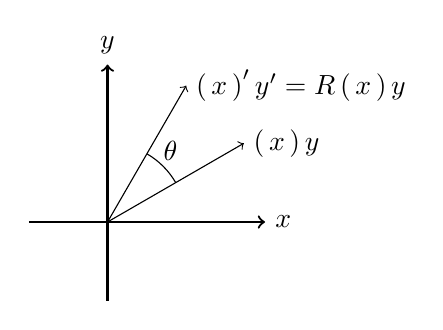
\begin{tikzpicture}
\draw[thick,->] (-1,0) -- (2,0)node[anchor=west] {$x$};
\draw[thick,->] (0,-1) -- (0,2)node[anchor=south] {$y$};
\draw (0.866,0.5) arc (30:60:1) ;
\draw[->] (0,0)--(1.732,1) node[right] {$\begin{pmatrix} x \\ y \end{pmatrix}$};
\draw[->] (0,0)-- (1,1.732) node[right] {$\begin{pmatrix} x '\\ y' \end{pmatrix}=R\begin{pmatrix} x \\ y \end{pmatrix}$};
\node at (0.8,0.9){$\theta$};
\end{tikzpicture}

\begin{Titre}
Pour une rotation anti-horaire autour de l'origine, on a  $x '= x \cos \theta -y \sin \theta$ et $y ' = x \sin \theta + y \cos \theta$ et sous la forme matricielle : $\begin{pmatrix} x '\\ y' \end{pmatrix} = R \begin{pmatrix} x \\ y \end{pmatrix}$ avec $R=\begin{pmatrix}
\cos \theta & -\sin \theta\\
\sin \theta & \cos \theta\\
\end{pmatrix}$
\end{Titre}
\end{Figure}
\end{center}
\end{Exemple}









\begin{Definition}[Endomorphisme]
\begin{itemize}
\item
  Une application linéaire dont l'espace de départ est le même que celui d'arrivée est un \defi{endomorphisme}.
\item
  Un \defi{isomorphisme} est une application linéaire bijective.
\item
  Un \defi{automorphisme} est un endomorphisme bijectif.
\end{itemize}
\end{Definition}
\begin{Exemple}
$\Phi _3$ et $R_\theta$ sont des endomorphismes. Comme $R_\theta$ est bijectif, $R_\theta$ est un automorphisme. 
\end{Exemple}
\begin{Texte}
Un isomorphisme permet de transporter les propriétés vectoriels entre les deux espaces vectoriels, par exemple la dimension.  Toute propriété ``vectorielle'' vraie pour un espace vectoriel donné sera vraie pour un espace vectoriel qui lui est isomorphe. \\
Par exemple, l'application linéaire $\Fonction{\phi}{\R_3}{\R_2[X]}{(a,b,c)}{a + bX + cX^2}$ est un isomorphisme qui "géométrise" $\R _2[X]$.
La coplanarité des vecteurs $(0, 1, 0)$, $(0, 0, 1)$ $(0, 1, \frac 1 2)$ et  se traduit dans $\R_2[X]$ par celle des vecteurs $X$, $X^2$ et $X +\frac 1 2  X^2$.
\begin{center}
\begin{Figure}
\begin{tikzpicture}
\draw[color=colordef,->] (0,0) -- (-0.7,-0.7)node[left] {$(1,0,0)$};
\draw[color=colordef,->] (0,0) -- (0.9,-0.2)node[right] {$(0,1,0)$};
\draw[color=colordef,->] (0,0) -- (0,1.2)node[above] {$(0,0,1)$};
\draw[color=colorprop,->] (0,0) -- (0.9,0.4)node[right] {$(0,1,\frac 1 2)$};
\draw[color=colordef,dashed] (0.9,-0.2) -- (0.9,0.4);
\draw[color=colordef,dashed] (0,0.6) -- (0.9,0.4);
\node at (-0.8,0.7){$\R_3$};
\draw[->](2.5,0.7)--node[above]{$\phi$}(4.5,0.7);
\begin{scope}[shift={(7,0)}]
\draw[color=colordef,->] (0,0) -- (-0.7,-0.7)node[left] {$1$};
\draw[color=colordef,->] (0,0) -- (0.9,-0.2)node[right] {$X$};
\draw[color=colordef,->] (0,0) -- (0,1.2)node[above] {$X^2$};
\draw[color=colorprop,->] (0,0) -- (0.9,0.4)node[right] {$X+\frac 1 2 X^2$};
\draw[color=colordef,dashed] (0.9,-0.2) -- (0.9,0.4);
\draw[color=colordef,dashed] (0,0.6) -- (0.9,0.4);
\node at (-0.8,0.7){$\R_2[X]$};
\end{scope}
\end{tikzpicture}
\end{Figure}
\end{center}
Aussi les isomorphismes nous permettent d'identifier deux espaces vectoriels, par exemple on identifie fréquemment les $p$-uplets avec les matrices colonnes 
car l'application
\[ \Fonction{\Phi }{\K ^p}{\M{p}{1}{\K}}{(\lambda_1,\dots,\lambda_p)}{\begin{pmatrix}\lambda_1\\\vdots\\\lambda_p\end{pmatrix}} \]
est un isomorphisme.\\
Par exemple, on notera $X=\begin{pmatrix}x_1\\x_2\\\end{pmatrix}\overbrace{=}^{\text{identification}}(x_1,x_2)=\Vect{x}.$
\end{Texte}










\begin{DefinitionProposition}[Espace vectoriel des application linéaires et endomorphismes]
Soit $E$ et $F$ deux $\K $-espaces vectoriels.
L'ensemble des applications linéaires de $E$ dans $F$ est noté \defi{$\mathcal{L}(E,F)$} ;
il s'agit d'un sous espace vectoriel de l'espace des fonctions de $E$ dans $F$ muni des lois usuelles.\\
L'espace vectoriel des endomorphismes de $E$ se note \defi{$\LE$}$= \mathcal{L}(E,E)$.
\end{DefinitionProposition}
\begin{Demonstration}
Tous les axiomes se vérifient aisément.  
\end{Demonstration}
\begin{Definition}[composition d'application linéaire]
La \defi{loi de composition interne $\circ$} est définie comme une composition de fonctions, c'est à dire si $u\in\mathcal{L}(E,F)$ et $v\in\mathcal{L}(F,G) $,
 alors  $\forall \Vect{x} \in E : (v\circ u)(\Vect{x})=v(u(\Vect{x}))$.\\
On a $v\circ u\in \mathcal{L}(E,G).$
 \end{Definition}
\begin{Exemple}
L'application $P\mapsto XP'(X^2)$ est un endomorphisme de $\K[X]$. Les applications $P\mapsto P'$, $P\mapsto P(X^2)$ et $P\mapsto XP$ sont linéaire, donc par composition  $P\mapsto XP'(X^2)$ l'est aussi.    
\end{Exemple} 
\begin{Definition}[Structure d'algèbre des endomorphismes]
L'\defi{élément neutre} de la composition dans $\LE$ est l'application identité, $Id_{E}:x\mapsto x$. L'endomorphisme $u^{-1}$ est appelé l' \defi{endomorphisme inverse} de $u$ si $ u^{-1}×u=u×u^{-1}=Id_{E}$. Dans ce cas, l'endomorphisme $u$ est dite \defi{inversible}.  $\LE$ possède une structure d'algèbre non commutative. L'espace vectoriel des automorphismes de $E$ se note $ \GLE$.   $(\GLE,\circ)$ est un groupe, appelé \defi{groupe linéaire}.
\end{Definition}

\subsection{Propriétés}
\begin{Proposition}[0 image de 0]
Soit $u:E\to F$ une application linéaire.\\
Alors $u(\Vect{0_E})=\Vect{0_F}$
\end{Proposition}
\begin{Demonstration}
$u(\Vect{0_E})\overbrace{=}^{\text{Elt neutre}}u(\Vect{0_E}+\Vect{0_E})\overbrace{=}^{\text{linéarité}}=u(\Vect{0_E})+u(\Vect{0_E})$. En ajoutant  $-u(\Vect{0_E})$ aux deux membres de l'égalité, on obtient $u(\Vect{0_E})=\Vect{0_F}$.
\end{Demonstration}
\begin{Exemple} 
L'application $f(x,y)\mapsto (x+y,1)$ n'est pas linéaire car $f(0,0)=(0,1).$ d'après la contraposée de la proposition précédente. 
\end{Exemple}
\begin{Proposition}[Caractérisation de la linéarité]
$u:E\to F$ est linéaire si et seulement si
$$\forall   \lambda  \in  \K , \forall   \Vect{x},\Vect{y}\in  E:\quad u(\lambda \Vect{x} +  \Vect{y}) = \lambda u(\Vect{x}) +  u(\Vect{y}).$$
\end{Proposition}
\begin{Demonstration}
\begin{itemize}
\item $(\Longrightarrow)$  soit $\lambda  \in  \K ,    \Vect{x},\Vect{y}\in E$
$$u(\lambda \Vect{x} +  \Vect{y})\overbrace{=}^{\text{additivité}}u(\lambda \Vect{x}) +  u(\Vect{y})\overbrace{=}^{\text{homogénéité}}\lambda u( \Vect{x}) +  u(\Vect{y}).$$
\item $(\Longleftarrow)$ 
\begin{itemize}
\item additivité : soit  $\Vect{x},\Vect{y}\in  E$. On a :
$$u(\Vect{x}+\Vect{y})=u(1\Vect{x}+\Vect{y})=1u(\Vect{x})+u(\Vect{y})=u(\Vect{x})+u(\Vect{y})$$
\item homogénéité : soit  $\Vect{x}\in  E,\lambda\in\K$. On a :
$$u(\lambda\Vect{x})=u(\lambda\Vect{x}+\Vect{0})=\lambda u(\Vect{x})+u(\Vect{0})\overbrace{=}^{u \text{ additive}}\lambda u(\Vect{x})+\Vect{0}=\lambda u(\Vect{x})$$
\end{itemize}
\end{itemize}
\end{Demonstration}

 \begin{Proposition}[Propriétés algébriques]
\begin{itemize}
\item
  \propri{Associativité} : $$(u \circ v) \circ w =u \circ( v \circ w).$$
\item
  \propri{Bilinéarité} : 
  $$ (\lambda u + \mu v) \circ w = \lambda u\circ w + \mu v\circ w\text{ et }u\circ (\lambda v+ \mu w) =\lambda u\circ v + \mu u\circ w.$$
\end{itemize}
\end{Proposition}
\begin{Demonstration}
La composition des fonctions est associative donc en particulier les fonctions linéaires aussi.\\
Les fonctions sont linéaires à gauche. En revanche, il faut l'hypothèse de linéarité pour la linéarité à droite. En effet, soit $\Vect{x}\in E$. On a :
$$u\circ (\lambda v+ \mu w)(\Vect{x})=u(\lambda v(\Vect{x})+ \mu w(\Vect{x}))\overbrace{=}^{\text{linéarité de }u}=\lambda u(v(\Vect{x})) + \mu u(w(\Vect{x})).$$
\end{Demonstration}

\begin{Remarque} On omet le plus souvent le symbole  $\circ$ : $v\circ u =v u$.
\end{Remarque}




%TODO mettre un exemple
\section{Image et noyau}
\subsection{Généralités}
\begin{Definition}[Image directe et image réciproque]
Soit $f:A\to B$. Soit $A'$ une partie de $A$ et $B'$ une partie de $B$.\\
L'ensemble $\{f(x): x  \in  A'\}$ est appelé \defi{image directe} de $A'$ par $f$ et noté $f(A')$.\\
L'ensemble $\{x\in A : f(x)  \in  B'\}$ est appelé \defi{image réciproque} de $B'$ par $f$ et noté $f^{-1}(B')$.\\
\end{Definition}
\begin{Exemple}[Carré]
Soit $f:x\mapsto x^2$.\\
On a $f([-1,1])=[0,1]$ et $f^{-1}(\{2\})=\{-\sqrt{2},\sqrt{2}\}$.
\end{Exemple}
\begin{Proposition}[Morphisme d'espace vectoriel]
Soit $E',F'$ deux sous-espace vectoriel de de $E$ et $F$ respectivement.
\begin{itemize}
\item $u(E')$ est un sous espace vectoriel de $F$,
\item $u^{-1}(F')$ est un sous espace vectoriel de $E$.
\end{itemize}
\end{Proposition}
\begin{Demonstration}
\begin{itemize}
\item 
\begin{itemize}
\item Non vide : Comme $u(\Vect{0_E})=\Vect{0_F}$, $\Vect{0_F}\in u(E')$.\\
\item Stabilité : Soit $\lambda\in\K, u(\Vect{x}),u(\Vect{x'})\in u(E')$.\\
On a $\lambda u(\Vect{x})+u(\Vect{x'})\overbrace{=}^{\text{linéarité}}u(\overbrace{\lambda\Vect{x}+\Vect{x'}}^{\in E'})\in u(E')$.\\
\end{itemize}
Ainsi $u(E')$ est un sous espace vectoriel de $F$.
\item 
\begin{itemize}
\item Non vide : comme $u(\Vect{0_E})=\Vect{0_F}\in F'$, $\Vect{0_E}\in u^{-1}(F')$.\\
\item Stabilité : soit $\lambda\in\K, \Vect{x},\Vect{x'}\in u^{-1}(F')$.\\
 On a $ u(\lambda\Vect{x}+\Vect{x'})\overbrace{=}^{\text{linéarité}}\lambda \overbrace{u(\Vect{x})}^{\in F'}+\overbrace{u(\Vect{x'}}^{\in F'}\in F'$. Donc $\lambda\Vect{x}+\Vect{x'}\in u^{-1}(F')$.
\end{itemize}
Ainsi $u^{-1}(F')$ est un sous espace vectoriel de $E$.
\end{itemize}
\end{Demonstration}


\begin{Exemple}
L'image de la droite vectoriel $\R (1,1)$ par $R_\theta$ est la droite vectoriel $\R R_\theta(1,1)$.

\begin{center}
\begin{Figure}
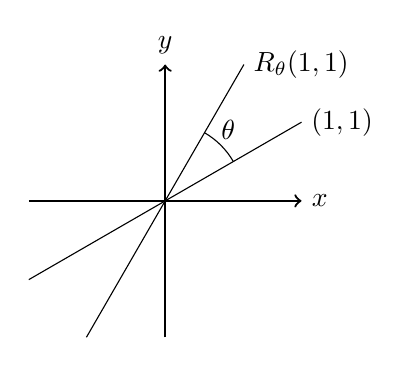
\begin{tikzpicture}
\draw[thick,->] (-1.732,0) -- (1.732,0)node[anchor=west] {$x$};
\draw[thick,->] (0,-1.732) -- (0,1.732)node[anchor=south] {$y$};
\draw (0.866,0.5) arc (30:60:1) ;
\draw[-] (-1.732,-1)--(1.732,1) node[right] {$\R (1,1)$};
\draw[-] (-1,-1.732)-- (1,1.732) node[right] {$\R R_\theta(1,1)$};
\node at (0.8,0.9){$\theta$};
\end{tikzpicture}
\end{Figure}
\end{center}

\end{Exemple}
\begin{Definition}[Image]

L'\defi{image} de $u$ est le sous espace vectoriel $u(E) = \{u(\Vect{x}):\Vect{x}\in  E\}$;
  on le note \defi{$\im u$}.\\
Par définition de la surjectivité, $\im u=E$ si et seulement $u$ est surjective. 
\end{Definition}
\begin{Definition}[Rang] Le \defi{rang} d'une  application linéaire $u$ est  la dimension de l'espace vectoriel $\Ima u$;
  on le note \defi{$\rg u$}.\\
\end{Definition}

\begin{Definition}[Noyau]
Le \defi{noyau} de $u$ est le le sous espace vectoriel $u^{-1}\{ \{\Vect{0_F}\}\} = \{x\in  E:u(\Vect{x}=\Vect{0_F}\}$;
on le note \defi{$\Ker u$}.
\end{Definition}

\begin{Proposition}[Caractérisation de l'injectivité par le noyau]  
$u$ est injective si et seulement si $\Ker u = \{\Vect{0_E}\}$.
\end{Proposition}

\begin{Demonstration}  
\begin{itemize}
\item Supposons que $u$ est injective.
 \begin{itemize}
\item $\Ker u \supset \{\Vect{0_E}\}$ : comme $\Ker u$ est un sous-espace vectoriel de $E$, il contient $\Vect{0_E}$
\item $\Ker u \subset \{\Vect{0_E}\}$ : soit $\Vect{x}\in \Ker u $. On a $u(\Vect{x})=\Vect{0_F}$. Comme $u$ est linéaire, $u(\Vect{0_E})=\Vect{0_F}$. Ainsi 
$u(\Vect{x})=u(\Vect{0_E})$. Comme $u$ est injective, $\Vect{x}=\Vect{0_E}$.
\end{itemize}
Du fait de la double inclusion $\Ker u = \{\Vect{0_E}\}$.
\item  Supposons que $\Ker u = \{\Vect{0_E}\}$.\\
soit $\Vect{x},\Vect{x'}\in E $ tel que $u(\Vect{x})=u(\Vect{x'})$. Alors $u(\Vect{x})-u(\Vect{x'})=\Vect{0_F}$ et par linéarité $u(\Vect{x}-\Vect{x'})=\Vect{0_F}$. Donc $\Vect{x}-\Vect{x'}\in \Ker u= \{\Vect{0_E}\}$. Ainsi $\Vect{x}-\Vect{x'}=\Vect{0_E}$. D'où $\Vect{x}=\Vect{x'}$.
\end{itemize}
\end{Demonstration}
\begin{Texte}
Pour démontrer une égalité entre deux ensembles, il faut prouver la double inclusion.    
En tant que sous-espace vectoriel de $E$, $\Ker u$ contient $\Vect{0}_E$, donc $\{\Vect{0}_E\}\subset \Ker u$. Ainsi démontrer que  $\Ker u = \{\Vect{0_E}\}$
et ainsi que $u$ est injective, il suffit en réalité de
montrer l'\impo{inclusion} : $\{\Vect{0_E}\}\subset \Ker u$.
\end{Texte}

\begin{Exemple}
Soit $\Fonction{u}{\R^3}{\R^2}{(x,y,z)}{(x+y+z,x-y)}$.\\
On a $u(x,y,z)=x(1,1)+y(1,-1)+z(0,1)$.
Donc $\Ima u$ est l'espace vectoriel engendré par la famille $((1,1),(1,-1),(0,1))$ d'où $\Ima u=\R^2$. Ainsi $u$ est surjective et $\rg u=2$.
$$(x,y,z)\in \Ker u \Leftrightarrow u(x,y,z)=(0,0)  \Leftrightarrow \begin{cases}x+y+z=&0\\x-y=&0\end{cases}\Leftrightarrow(x,y,z)=x(1,1,-2).$$
Donc $\Ker u =\R (1,1,2).$ Ainsi $u$ n'est pas injective.
\end{Exemple}
\begin{Exemple}[Dérivée polynomiale]
Soit $P=a_0+a_1 X+\dots + a_n X^n \in \R_n[X].$
On a $\Phi_3(P)=P'=a_1+a_2 .2X+\dots  + a_n.nX^{n-1}$.
Donc $\Ima \Phi_3$ est l'espace vectoriel engendré par la famille $(1,X,2X,\dots,nX^{n-1})$, soit $\Ima \Phi_3=\R_{n-1}[X].$ $\Phi_3$ n'est pas surjective $\rg u=\dim \R_{n-1}[X]=n $.
 $$P\in \Ker \Phi_3  \Leftrightarrow \Phi_3(P)=0  \Leftrightarrow P'=0\Leftrightarrow \exists a\in \R : P=a.$$
Donc $\Ker \Phi_3 =\R_{0}[X].$ $\Phi_3$ n'est pas injective.
\end{Exemple}




\begin{Proposition}[Permutation de Vect et de l'image]
Soit $(\Vect{x_i})_{i\leq i \leq n }$ une famille de $E$ .\\
Alors $$ u(\text{Vect}((\Vect{x_i})_{i\leq i \leq n}))=\text{Vect}\left(u(\Vect{x_i})\right)_{i\leq i \leq n}.$$
\end{Proposition}
\begin{Demonstration}
\begin{itemize}
\item  $u(\text{Vect}((\Vect{x_i})_{i\leq i \leq n}))\subset\text{Vect}\left(u(\Vect{x_i})\right)_{i\leq i \leq n}$:\\
Soit $\sum_{i=1}^n \lambda_i \Vect{x_i}\in \text{Vect}((\Vect{x_i})_{i\leq i \leq n})$.\\
Comme $u(\sum_{i=1}^n \lambda_i \Vect{x_i})\overbrace{=}^{\text{linéarité}}\sum_{i=1}^n \lambda_i u( \Vect{x_i})$, $u(\sum_{i=1}^n \lambda_i \Vect{x_i})$ s'exprime comme combinaison linéaire des vecteurs $\left(u(\Vect{x_i})\right)_{i\leq i \leq n}$ donc appartient à $\text{Vect}\left(u(\Vect{x_i})\right)_{i\leq i \leq n}$
\item $u(\text{Vect}((\Vect{x_i})_{i\leq i \leq n}))\supset\text{Vect}\left(u(\Vect{x_i})\right)_{i\leq i \leq n}$: Raisonnement similaire.
\end{itemize}
Du fait de la double inclusion, on a bien $ u(\text{Vect}((\Vect{x_i})_{i\leq i \leq n}))=\text{Vect}\left(u(\Vect{x_i})\right)_{i\leq i \leq n}.$
\end{Demonstration}
\begin{Corollaire}[Image d'une base]
Soit $(\Vect{e_i})_{i\leq i \leq n}$ une base de $E$ .\\
Alors $$ \Ima u =\text{Vect}( \left(u(\Vect{x_i})\right)_{i\leq i \leq n})).$$
\end{Corollaire}
\begin{Demonstration}
Comme $ \Ima u =u(E)$ et $E=\text{Vect}(\Vect{e_i})_{i\leq i \leq n }$, d'après la proposition précédente, on obtient $ \Ima u =\text{Vect}( \left(u(\Vect{x_i})\right)_{i\leq i \leq n})).$
\end{Demonstration}

\begin{Proposition}[Linéarité de l'inverse]
Si $u$ est un isomorphisme, alors $u^{-1}$ est également linéaire.
\end{Proposition}
\begin{Demonstration}  
Soit $\Vect{x},\Vect{x'}\in F $ et $\lambda\in\K$.\\
On a $u(u^{-1}(\lambda\Vect{x}+\Vect{x'}))=\lambda\Vect{x}+\Vect{x'}$. De plus, $u(\lambda u^{-1}(\Vect{x})+ u^{-1}(\Vect{x'}))\overbrace{=}^{\text{linéarité}}\lambda u( u^{-1}(\Vect{x}))+ u(u^{-1}(\Vect{x'}))=\lambda\Vect{x}+\Vect{x'}.$. Ainsi $u(u^{-1}(\lambda\Vect{x}+\Vect{x'}))=u(\lambda u^{-1}(\Vect{x})+ u^{-1}(\Vect{x'}))$. Comme $u$ est injective,  $u^{-1}(\lambda\Vect{x}+\Vect{x'})=\lambda u^{-1}(\Vect{x})+ u^{-1}(\Vect{x'})$.\\
 $u^{-1}$ est donc linéaire.
\end{Demonstration}





\subsection{Effet d'une applications linéaire sur la dimension}
\begin{Texte}
Une application linéaire, $u:E\to F$ ne peut que réduire la dimension de son ensemble de définition. 
\begin{center}
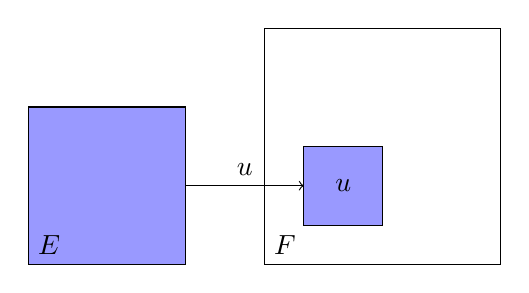
\begin{tikzpicture}
\fill[blue!40!white, draw=black] (0,0) rectangle (2,2);
\draw  (0,0) node[above right]{$E$};
\fill[white, draw=black] (3,0) rectangle (6,3);
\draw  (3,0) node[above right]{$F$};
\fill[blue!40!white, draw=black] (3.5,0.5) rectangle (4.5,1.5);
\draw  (4,1) node{$\im u$};
\draw[->]  (2,1) --node[above]{$u$} (3.5,1) ;
\end{tikzpicture}
\end{center}
L'application est injective si et seulement si: $\rg u =\dim E$.
\begin{center}
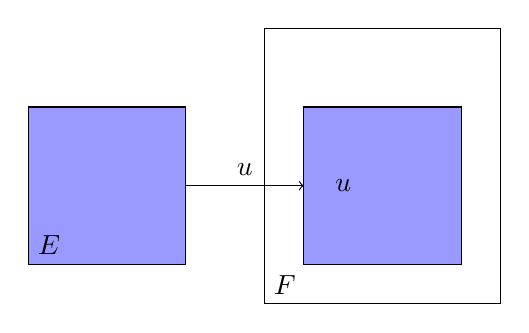
\begin{tikzpicture}
\fill[blue!40!white, draw=black] (0,0) rectangle (2,2);
\draw  (0,0) node[above right]{$E$};
\fill[white, draw=black] (3,-0.5) rectangle (6,3);
\draw  (3,-0.5) node[above right]{$F$};
\fill[blue!40!white, draw=black] (3.5,0) rectangle (5.5,2);
\draw  (4,1) node{$\im u$};
\draw[->]  (2,1) --node[above]{$u$} (3.5,1) ;
\end{tikzpicture}
\end{center}
L'application est surjective si et seulement si: $\rg u =\dim F$.
\begin{center}
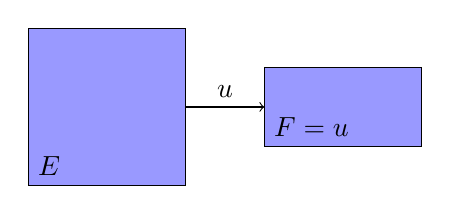
\begin{tikzpicture}
\fill[blue!40!white, draw=black] (0,0) rectangle (2,2);
\draw  (0,0) node[above right]{$E$};
\fill[blue!40!white, draw=black] (3,0.5) rectangle (5,1.5);
\draw  (3,0.5) node[above right]{$F=\im u$};
\draw[->]  (2,1) --node[above]{$u$} (3,1) ;
\end{tikzpicture}
\end{center}
L'application est un isomorphisme si et seulement si: $\rg u =\dim F=\dim E$.
\begin{center}
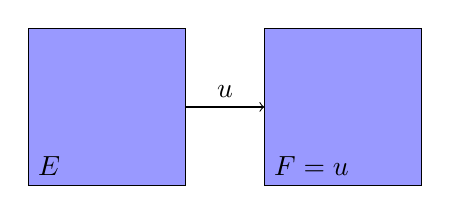
\begin{tikzpicture}
\fill[blue!40!white, draw=black] (0,0) rectangle (2,2);
\draw  (0,0) node[above right]{$E$};
\fill[blue!40!white, draw=black] (3,0) rectangle (5,2);
\draw  (3,0) node[above right]{$F=\im u$};
\draw[->]  (2,1) --node[above]{$u$} (3,1) ;
\end{tikzpicture}
\end{center}
\end{Texte}
\begin{Proposition}[Inégalité et égalité sur le rang]
Soit $u:E\to F$ une application linéaire.
\begin{itemize}
\item Si $F$ est de dimension finie, alors $\rg u \leq \dim F$, avec égalité si et seulement si $u$ est surjective.
\item  Si $E$ est de dimension finie, alors $\rg u \leq \dim E$, avec égalité si et seulement si $u$ est injective.
\end{itemize}
\end{Proposition}
\begin{Demonstration}
\begin{itemize}
\item 
Comme $\im u \subset F$, on a $\rg u =\dim  \im u\leq \dim F$. Pour l'égalité, on a  $u$ est surjective si et seulement si  $\im u =  F$ si et seulement si $\dim  \im u\leq \dim F$.
\item Soit $n$ la dimension de $E$ et $(\Vect{e_1},\dots,\Vect{e_n})$ une base de $E$. Comme $\im u=\operatorname{Vect}(u(\Vect{e_1}),\dots,u(\Vect{e_n}))$, $\dim  \im u\leq n$. Pour l'égalité, on a $\rg u \leq \dim E$ si et seulement si $u(\Vect{e_1}),\dots,u(\Vect{e_n})$ est une famille libre de $F$. 
\begin{itemize}
\item 
Supposons que $(u(\Vect{e_1}),\dots,u(\Vect{e_n}))$ est une famille libre de $F$. \\
Soit $\Vect{x}=\sum_{i=1}^n x_i\Vect{e_i} \in \Ker u$.
$$
\begin{aligned}
u(\vec{x})&=\Vect{0_F}&\\
u(\sum_{i=1}^n x_i\vec{e_i})&=\Vect{0_F}&\\
\sum_{i=1}^n x_i u(\vec{e_i})&=\Vect{0_F}&\text{ car u  linéaire}\\
\forall i\in \Intf{1}{n}:\quad x_i=0 &&\text{ car }  (u(\vec{e_1}),\dots,u(\vec{e_n})) \text{ libre}\\
\Vect{x}=\sum_{i=1}^n x_i\Vect{e_i}&=\Vect{0_E}&
\end{aligned}.
$$ Ainsi $\Ker u\subset \{\Vect{0_E}\}$. Donc $u$ est injective.
\item Supposons que $u$ est injective.\\
Soit $\lambda_1,\dots,\lambda_n\in\K$ tel que 
$$
\begin{aligned}
\sum_{i=1}^n\lambda_i u(\vec{e_i}))&=\Vect{0_F}&\\
u(\sum_{i=1}^n\lambda_i \vec{e_i}))&=\Vect{0_F}&\text{ car u  linéaire}\\
\sum_{i=1}^n\lambda_i \vec{e_i} &=\Vect{0_E}&\text{ car u  }\Ker u= \{\vec{0_E}\}\\
\forall i\in \Intf{1}{n}:\quad \lambda_i=0 &&\text{ car }  (\vec{e_1},\dots,\vec{e_n}) \text{ libre}\\
\end{aligned}.
$$
Donc $(u(\Vect{e_1}),\dots,u(\Vect{e_n}))$ est une famille libre de $F$.
\end{itemize}
\end{itemize}
\end{Demonstration}


\begin{Proposition}[Cas $\dim E = \dim F$]
Soit $u:E\to F$ une application linéaire tel que $\dim E = \dim F$.
\begin{center}
$u$ est un isomorphisme $\Leftrightarrow$ $u$ est injective $\Leftrightarrow$ $u$ est surjective.
\end{center}
Soit $u:E\to E$ une application linéaire tel que $\dim E$ est finie.
\begin{center}
\begin{tabular}{ccccc}
$u$ est un isomorphisme& $\Leftrightarrow$& $u$ est injective &$\Leftrightarrow$ &$u$ est surjective \\
$u\in \mathcal{GL}(E)$ &$\Leftrightarrow$ &  $u$ est inversible à gauche &$\Leftrightarrow$ &  $u$ est inversible à droite \\
$\exists v\in \LE: u\circ v =v \circ u = \mathrm{Id}_E$ &$\Leftrightarrow$ &  $\exists v\in \LE: v\circ u= \mathrm{Id}_E$  &$\Leftrightarrow$ &  $\exists v\in \LE: u\circ v= \mathrm{Id}_E$
\end{tabular}
\end{center}
\end{Proposition}

\begin{Demonstration}
\begin{itemize}
\item  Par hypothèse $\dim E = \dim F$. On a $u$ est injective si et seulement si : $\rg u = \dim E$ si et seulement si $\rg u = \dim F$   si et seulement si $u$ est surjective.
\item $u$ est inversible à gauche  si et seulement si  $\exists v\in \LE: v\circ u= \mathrm{Id}_E$   si et seulement si $u$ est injective si et seulement si $u$ est surjective  si et seulement si $\exists v\in \LE: u\circ v= \mathrm{Id}_E$ si et seulement si $u$ est inversible à droite.
\end{itemize}
\end{Demonstration}

\begin{Exemple}
Démontrer que l'application linéaire $\Fonction{u}{\R^2}{\R^2}{(x,y)}{ (x+y,x-y)}$ est un automorphisme.
\begin{Demonstration}
Comme $u$ est un endomorphisme, il suffit de démontrer qu'elle est injective.\\
$$(x,y)\in \Ker u \Leftrightarrow \begin{cases}x+y=0\\x-y=0\end{cases}  \Leftrightarrow  \begin{cases}x=0\\y=0\end{cases} $$ 
Donc $\Ker u =\{(0,0)\}.$
\end{Demonstration}
\end{Exemple}
\begin{Exemple}
Démontrer que l'application linéaire $\Fonction{u}{\R_n[X]}{\R_n[X]}{P}{  P-P}$  est un automorphisme.
\begin{Demonstration}
Comme $u$ est un endomorphisme, il suffit de montrer qu'elle est injective.\\
$$P\in \Ker u \Leftrightarrow P-P'=0  \Leftrightarrow  P=P'$$ 
Donc $\Ker u =\{0\}$ car $\deg(P)=\deg(P')$ si et seulement $P=0$.
\end{Demonstration}
\end{Exemple}

\subsection{Théorème du rang : $\dim E = \Rang u + \dim \Ker u$}
%Les dimensions du noyau et l'image d'une application linéaire sont liées.\\
%Soit $A=\begin{pmatrix} 1 &  0 &1\\ 0 &1 &1\\ 0 &1&1\end{pmatrix}$. On a $C_3=C_1+C2$.\\
%\textit{Image}  : $\im(A)=\mathrm{Vect}(C_1,C_2,C_3)\overbrace{=}^{C_3=C_1+C2}\mathrm{Vect}(C_1,C_2).$ Comme les vecteur $C_1$ et $C_2$ sont linéairement indépendants, $\dim (\im(A))=2$.\\
%\textit{Noyau}  : $\begin{pmatrix}x\\y\\z \end{pmatrix}\in \Ker(A)\Leftrightarrow xC_1 + yC_2 + zC_3= 0\overbrace{\Leftrightarrow}^{C_3=C_1+C2} (x+z)C_1 + (y+z)C_2 = 0$ \\$ \overbrace{\Leftrightarrow}^{C_1,C_2\text{linéairement indépendants} }\begin{cases}x=-z\\y=-z\end{cases} \Leftrightarrow \Ker(A)= \mathrm{Vect} \begin{pmatrix}1\\1\\-1 \end{pmatrix}$. Donc $\dim (\Ker(A))=1$.\\
%On observe que $\dim \Ker A +\dim \im A =$taille de la matrice. 

\begin{Texte}
 le théorème du rang lie le rang d'une application linéaire et la dimension de son noyau.
\end{Texte}
\begin{Lemme}[Factorisation]
Soit $E$ et $F$ deux $\K $-espaces vectoriels  et $u:E\to F$ une application linéaire.
Si $S$ est un supplémentaire de $\Ker u$, \\
Alors $u$ induit un isomorphisme de $S$ sur $\Ima u$,
c'est à dire que l'application linéaire
\[ \Fonction{u\vert_S}{S}{\Ima u}{\vec{x}}{u(\vec{x})} \]
est un isomorphisme.
\end{Lemme}
\begin{Demonstration}
\begin{itemize}
\item Injective :  Soit $\Vect{x}\in\Ker u\vert_S$ donc $x\in\Ker u$ et  $x\in S$. Comme $\Ker u$ et  $S$ sont supplémentaires, $\Ker u \cap S =\{\Vect{0_E}\}$. D'où $\Vect{x}=\Vect{0_E}$ et $\Ker u\vert_S=\{\Vect{0_E}\}$. 
\item Surjective : Soit $\Vect{y}\in \im u$ ainsi il existe $\Vect{x}\in E$ tel que $u(\Vect{x})=\Vect{y}$.  Comme  $\Ker u$ et  $S$ sont supplémentaires, il existe $\Vect{k}\in\Ker u$  et $\Vect{s}\in S $ tel que $\Vect{x}=\Vect{k}+\Vect{s}$. On  a :
$$
\begin{aligned}
u(\vec{x})&=\vec{y}&\\
u(\vec{k}+\vec{s})&=\vec{y}&\\
u(\vec{k})+u(\vec{s})&=\vec{y}&\text{ car u  linéaire}\\
 u(\vec{s})&=\vec{y}&\text{ car } \Vect{k}\in\Ker u.\\
\end{aligned}
$$
Ainsi $\Vect{s}$ est un antécédent de $\Vect{y}$ par l'application $u\vert_S$. Donc $u\vert_S$ est surjective.
\end{itemize}
\end{Demonstration}

\begin{Theoreme}[Théorème du rang]

Soit $E$ et $F$ deux $\K $-espaces vectoriels  et $u:E\to F$ une application linéaire.
On suppose que $E$ est de dimension finie.
Alors $\Ima u$ est de dimension finie et
\[ \dim E = \Rang u + \dim \Ker u. \]
\end{Theoreme}

\begin{Demonstration}
Comme $E$ est de dimension finie, $\Ker u$ possède un supplémentaire $S$ dans $E$. D'après le lemme de factorisation, comme $u\vert_S$ 
est un isomorphisme,   $\dim S = \dim \im u$. Comme  $S$ et $\Ker u$ sont supplémentaires dans $E$, on a $\dim S+\dim \Ker u=\dim E$. Finalement, on a 
$\dim \im u+\dim \Ker u=\dim E$.
\end{Demonstration}
%TODO exercices http://uel.unisciel.fr/mathematiques/espacevect1/espacevect1_ch04/co/apprendre_ch4_07_07.html et redémontrer effet d'une application linéaire 
\section{Dualité entre le point vue application linéaire et le  point de vue matriciel en dimension finie}

\subsection{Représentation matricielle d'une application linéaire}
Dans cette sous-section, tous les espaces vectoriels sont de dimension finie.\\
\begin{Definition}[Coordonnées d'un vecteur]
Soit $\mathcal{B} = (\Vect{e_1},\dots,\Vect{e_p})$ une base de $E$.\\
On sait que tout vecteur $\Vect{x}\in  E$ se décompose de façon unique sous la forme
$\Vect{x} = x_1 \Vect{e_1} + \dots + x_p \Vect{e_p}$ où $x_1,\dots, x_p \in   \K$.\\
On appelle coordonnées de $\Vect{x}$ dans la base $E$ la matrice colonne
\[ [\Vect{x}]_\mathcal{B} = \begin{pmatrix}
x_1\\\vdots\\x_p\\
\end{pmatrix} \]
\end{Definition}


\begin{Exemple}[Polynôme] 
Soit $P=1-X^2\in \R_n[X]$. Dans la base canonique $\mathcal{B}=(1,X,X^2,\dots,X^n)$ de $\R_n[X]$, on a $$[P]_\mathcal{B}=\begin{pmatrix}1\\0\\-1\\0\\\vdots \\0\\\end{pmatrix}$$. 
\end{Exemple}
\begin{Definition}[Matrice d'une application linéaire]
Soit $\mathcal{B} = (\Vect{e_1},\dots,\Vect{e_p})$ une base de $E$ et $\mathcal{B}' = (\Vect{f_1},\dots,\Vect{f_n})$ une base de $F$.
Pour tout $j\in  \{1,\dots,p\}$, le vecteur $u(\Vect{e_j})$ se décompose dans la base $\mathcal{B}'$:
\[u(\Vect{e_j})=a_{1j}.\Vect{f_1}+\dots +a_{nj}.\Vect{f_n}. \]
On appelle \defi{matrice de l'application linéaire $u$} la matrice, $[u]_\mathcal{B}^{\mathcal{B}'}$,  définie par :
\begin{center}
  \begin{tikzpicture}[
      every left delimiter/.style={xshift=0.75em},
      every right delimiter/.style={xshift=-0.75em},
      dots/.style={
        line width=1pt,
        line cap=round,
        dash pattern=on 0pt off 5pt,
        shorten >=.1cm,
    shorten <=.1cm}]
    \matrix (M) [
      matrix of nodes,
      left delimiter=(,
      right delimiter=),
    ]{
      \node (A) {$a_{11}$}; &[1.1cm] \node (B) {$a_{1p}$}; \\[1.1cm]
      \node (C) {$a_{n1}$}; &        \node (D) {$a_{np}$}; \\
    };

    \draw (M.west) node[left] {$[u]_\mathcal{B}^{\mathcal{B}'}=$};
    \draw [dots] (A.east)  -- (B.west);
    \draw [dots] (C.east)  -- (D.west);
    \draw [dots] (A.south) -- (C.north);
    \draw [dots] (B.south) -- (D.north);
    \draw (A) [yshift=0.7cm] node (E) {$u(\Vect{e_1})$};
    \draw (B) [yshift=0.7cm] node (F) {$u(\Vect{e_p})$};
    \draw (B) [xshift=1cm]   node (G) {$\Vect{f_1}$};
    \draw (D) [xshift=1cm]   node (H) {$\Vect{f_n}$};
    \draw [dots] (E.east)  -- (F.west);
    \draw [dots] (G.south) -- (H.north);
  \end{tikzpicture}
\end{center}
Les autres notations sont $ [u]_\mathcal{B}^{\mathcal{B}'}= \mat(u,\mathcal{B} \to \mathcal{B}') = \mat_{\mathcal{B}\to\mathcal{B}'}(u).$\\
Dans le cas d'un endomorphisme, $E=F$  et $\mathcal{B}=\mathcal{B}'$, on la note $[u]_\mathcal{B}$ ou $\mat(u,\mathcal{B})$ ou $\mat_\mathcal{B}(u)$.
\end{Definition}
\begin{Exemple}[Dérivée polynomial] La matrice de $\Fonction{\Phi _3}{\mathbb {R}_n[X] }{\mathbb {R}_n[X]}{P}{P'}$ dans la base canonique $\mathcal{B}=(1,X,X^2,\dots,X^n)$ est :
 $$[\Phi _3]_{\mathcal{B}}= \begin{pmatrix} 0 &1&0&\ldots &0 \\
 0& 0&2&\ddots \\
 \vdots &  &\ddots & \ddots \\
  \vdots &  & & \ddots& n\\
 0 &  & \dots& & 0
\end{pmatrix}   $$
car $\Phi _3(X^i)=i X^{i-1}$.
\end{Exemple}


\begin{Theoreme}[Image d'une application linéaire et image d'une matrice]
Soit $\mathcal{B}$ une base de $E$ et $\mathcal{B}'$ une base de $F$.\\
Soit $u:E\to F$ une application linéaire et $\Vect{x}$ un vecteur de $E$.\\
Alors \[ [u(\Vect{x})]_{\mathcal{B}'} = [u]_\mathcal{B}^{\mathcal{B}'} × [\Vect{x}]_\mathcal{B}. \]
ou si on pose $Y=[u(\Vect{x})]_{\mathcal{B}'},\quad A =[u]_\mathcal{B}^{\mathcal{B}'}$ et  $[\Vect{x}]_\mathcal{B}$, on a :
$$Y=AX.$$
\end{Theoreme}
\begin{Demonstration}
Soit $\mathcal{B}=(\Vect{e_1},\dots,\Vect{e_p})$ une base de $E$.\\
Soit $\mathcal{B}'=(\Vect{f_1},\dots,\Vect{f_n})$ une base de $F$.\\
Soit $(a_{ij})_{\substack{1\leq i\leq n\\1\leq j\leq p}}$ les coefficients de la matrice $[u]_\mathcal{B}^{\mathcal{B}'}$.\\
Soit $\Vect{x}=x_1\Vect{e_1}+\dots+x_p\Vect{e_p}\in E$.\\
On a :
$$u(\Vect{x})\overbrace{=}^{\text{linéarité}} =\sum_{j=1}^p x_j\Vect{e_j}=\sum_{j=1}^p x_j\sum_{i=1}^n a_{ij} \Vect{f_i}=\sum_{i=1}^n \left(\sum_{j=1}^p x_j a_{ij}\right) \Vect{f_i}, $$
d'où $ [u(\Vect{x})]_{\mathcal{B}'}=\begin{pmatrix}\sum_{j=1}^p x_j a_{1j} \\\vdots\\\sum_{j=1}^p x_j a_{nj} \end{pmatrix}$.\\
Aussi on a :

$$\begin{aligned}\\
 &\begin{pmatrix}x_1\\\vdots\\x_p\end{pmatrix} \\
\left[u\right]_{\mathcal{B}}^{\mathcal{B}'} \times \left[\vec{x}\right]_{\mathcal{B}}=\begin{pmatrix}
    a_{11} &  \dots & a_{1p}  \\
    \vdots &   &  \vdots  \\
    a_{n1} &  \dots & a_{np}
  \end{pmatrix}& \\
\left[u\right]_{\mathcal{B}}^{\mathcal{B}'} \times \left[\vec{x}\right]_{\mathcal{B}}=\begin{pmatrix}\sum_{j=1}^p x_j a_{1j} \\\vdots\\\sum_{j=1}^p x_j a_{nj} \end{pmatrix}&.
\end{aligned}$$
Finalement on obtient bien $ [u(\vec{x})]_{\mathcal{B}'} = [u]_\mathcal{B}^{\mathcal{B}'} × [\Vect{x}]_\mathcal{B}. $
\end{Demonstration}

\begin{Exemple}[Dérivée polynomial] 
Soit $P=1-X^2$. On a $[P]_\mathcal{B}=\begin{pmatrix}1\\0\\-1\\0\\\vdots \end{pmatrix}$. D'où 
$$[\Phi_3(P)]_\mathcal{B}=  [\Phi _3]_{\mathcal{B}} [P]_\mathcal{B} =\begin{pmatrix} 0 &1&0&\ldots &0 \\
 0& 0&2&\ddots \\
 \vdots &  &\ddots & \ddots \\
  \vdots &  & & \ddots& n\\
 0 &  & \dots& & 0
\end{pmatrix}  \begin{pmatrix}1\\0\\-1\\0\\\vdots \end{pmatrix} = \begin{pmatrix}0\\-2\\0\\0\\\vdots \end{pmatrix}    $$
D'où le résultat escompté $\Phi_3(P)=-2X$.
\end{Exemple}

\begin{Theoreme}[Produit matriciel et composition d'applications linéaires]
Soit $E$, $F$, $G$ trois espaces vectoriels de dimension finie munis des bases respectives $\mathcal{B}$, $\mathcal{B}'$ et $\mathcal{B}''$.\\
Soit $u:E\to F$ et $v:F\to G$ deux applications linéaires.\\
Alors
$$  [v\circ u]_{\mathcal{B}}^{\mathcal{B}''} = [v]_{\mathcal{B}'}^{\mathcal{B}''} \times [u]_{\mathcal{B}}^{\mathcal{B}'}. $$
\end{Theoreme}

\begin{Demonstration}
Soit $\vec{x}\in E$. On a:
$$  [v\circ u]_{\mathcal{B}}^{\mathcal{B}''}[\vec{x}]_B=[v\circ u(\vec{x})]_{\mathcal{B}''} $$
et
$$  [v]_{\mathcal{B}'}^{\mathcal{B}''} \times [u]_{\mathcal{B}}^{\mathcal{B}'}[\vec{x}]_B=[v]_{\mathcal{B}'}^{\mathcal{B}''}[u(\vec{x})]_{\mathcal{B}'}=[v( u(\vec{x}))]_{\mathcal{B}''} $$
Ainsi les matrices $[v\circ u]_{\mathcal{B}}^{\mathcal{B}''}$ et $[v]_{\mathcal{B}'}^{\mathcal{B}''} \times [u]_{\mathcal{B}}^{\mathcal{B}'}$ sont égales. 
\end{Demonstration}
\begin{Definition}[Application linéaire d'une matrice]
Inversement, si l'on se donne une matrice $M \in   \M{n}{q}{\K} $,
on peut définir une application linéaire, dite \defi{canoniquement associée à $M$}, par
\[ \Fonction{u_M}{\M{p}{1}{\K}}{\M{n}{1}{\K}}{X}{M\times X}.\]
Si l'on note $\mathcal{B}$ la base canonique de $\M{p}{1}{\K}$ et $\mathcal{B}'$ la base canonique de $\M{n}{1}{\K}$,
on vérifie  que
\[ [u_M]_{\mathcal{B}}^{\mathcal{B}'} = M. \]
\end{Definition}

\begin{Exemple}[Matrice de rotation]
La matrice de rotation $\begin{pmatrix}\cos \theta & -\sin \theta\\ \sin \theta & \cos \theta\end{pmatrix}$ est canoniquement associée à l'application linéaire rotation $$\Fonction{R_\theta}{\mathbb {R}^2 }{\mathbb {R}^2}{(x,y)}{ (x\cos \theta - y \sin \theta,x\sin \theta + y \cos \theta)}.$$ 
\end{Exemple}



En résumé, soit  $\mathcal{B}=(\Vect{e}_1, \dots  ,\Vect{e}_p)$ et  $\mathcal{B}'=(\Vect{f}_1, \dots  ,\Vect{f}_n)$ bases de $E$ et $F$ respectivement, nous avons :\\
\begin{center}
\begin{tabular}{c|c|c}
Vectoriel &  &Matriciel \\
\hline\hline
$\Vect{x}=x_1.\Vect{e}_1+ \dots  +x_p.\Vect{e}_p \in E$& $\longrightarrow$ & $X=[\Vect{x}]_{\mathcal{B}}=\begin{pmatrix}x_1\\ \vdots\\x_p\end{pmatrix}\in\K^p $ \\\hline
$u\in\mathcal{L}(E,F)$ &$\longrightarrow$    & \begin{tikzpicture}[
      every left delimiter/.style={xshift=0.75em},
      every right delimiter/.style={xshift=-0.75em},
      dots/.style={
        line width=1pt,
        line cap=round,
        dash pattern=on 0pt off 5pt,
        shorten >=.1cm,
    shorten <=.1cm}]
    \matrix (M) [
      matrix of nodes,
      left delimiter=(,
      right delimiter=),
    ]{
      \node (A) {$a_{11}$}; &[1.1cm] \node (B) {$a_{1n}$}; \\[1.1cm]
      \node (C) {$a_{n1}$}; &        \node (D) {$a_{nn}$}; \\
    };

    \draw (M.west) node[left] {$A=[u]_\mathcal{B}=$};
    \draw [dots] (A.east)  -- (B.west);
    \draw [dots] (C.east)  -- (D.west);
    \draw [dots] (A.south) -- (C.north);
    \draw [dots] (B.south) -- (D.north);
    \draw (A) [yshift=0.7cm] node (E) {$u(\Vect{e_1})$};
    \draw (B) [yshift=0.7cm] node (F) {$u(\Vect{e_p})$};
    \draw (B) [xshift=1cm]   node (G) {$\Vect{f_1}$};
    \draw (D) [xshift=1cm]   node (H) {$\Vect{f_n}$};
    \draw [dots] (E.east)  -- (F.west);
    \draw [dots] (G.south) -- (H.north);
  \end{tikzpicture}\\\hline
$\Vect{y}=y_1.\Vect{f}_1+ \dots  +y_n.\Vect{f}_n=u(\Vect{x})$&$\longrightarrow$ & $Y=[\Vect{y}]_{\mathcal{B}'}=\begin{pmatrix}y_1\\ \vdots\\y_n\end{pmatrix}=A\times X $ \\\hline
 $u\circ v $ avec $u,v \in\LE$ &$\longrightarrow$ &  $[u\circ v]_{\mathcal{B}} =A\times B$ avec $A=[u]_\mathcal{B}$ et $B=[v]_\mathcal{B}$\\
%$\ker u = \{\Vect{x}\in E:u(\Vect{x}) = \Vect{0}\} $      &$\longrightarrow$ &$\ker [u]_\mathcal{B}= \{X:[u]_\mathcal{B} X = 0\}$ \\\hline
%$\im u = \{u(\Vect{x}):\Vect{x}\in E\} $      & $\longrightarrow$&$\im [u]_\mathcal{B}= \{[u]_\mathcal{B} X:X\in \M{M}{n,1}{\K}\}$\\\hline
\hline

$\Fonction{u_M}{ \K^p}{ \K^n}{X}{M\times X}   $ &$\longleftarrow $ & $M\in \M{n}{p}{\K}$
 
\end{tabular}
 \end{center}


 \subsection{Dualité entre la représentation matricielle et l'application linéaire}
\begin{Theoreme}[Caractérisation par l'image d'une base]
Pour connaître/définir une application linéaire complètement, il suffit de connaître/définir les  images d'une base de l'espace vectoriel de départ. 
\end{Theoreme}
\begin{Remarque}
Pour déterminer une application quelconque, on n'a pas d'autre choix que de déterminer les images de chaque point $x\mapsto f(x)$. En revanche,   une application linéaire est complètement déterminer par l'image d'une base. Par exemple, soit $u:(x,y)\mapsto u(x,y)$ une application linéaire avec les images de base canonique : $u(1,0)=(1,1)$ et $u(0,1)=(1,-1)$. On a 
$$u(x,y)=u(x(1,0)+y(0,1))\overbrace{=}^{\text{linéarité}}x.u(1,0)+ y.u(0,1)=x.(1,1)+ y.u(1,-1)=(x+y,x-y).$$    
\end{Remarque}
\begin{Demonstration}
Soit $\mathcal{B}=(\Vect{e_1},\dots,\Vect{e_p})$ une base de $E$.\\
Comme $u$ est linéaire, on a :
\begin{align}
u(\Vect{x})&=u(\lambda_1.\Vect{e_1}+\dots +\lambda_p.\Vect{e_p})\\
u(\Vect{x})&=\lambda_1.u(\Vect{e_1})+\dots +\lambda_p.u(\Vect{e_p})
\end{align}
Cela implique que l'application linéaire $u$ est entièrement déterminée par les vecteurs $(u(\Vect{e_1}),\dots,u(\Vect{e_p}))$.
\end{Demonstration}
\begin{Theoreme}[Dualité]
Soit $\mathcal{B}$ une base de $E$ et $\mathcal{B}'$ une base de $F$.\\
L'application
\[ \Fonction{\Phi}{\mathcal{L}(E,F)}{\M{n}{q}{\K} }{u}{[u]_\mathcal{B}^{\mathcal{B}'}} \]
est  un isomorphisme.
\end{Theoreme}
\begin{Demonstration}
On ajoute une seconde partie à la démonstration sur la caractérisation d'une application linéaire par l'image d'une base.\\
Soit $\mathcal{B}'=(\Vect{f_1},\dots,\Vect{f_n})$ une base de $F$.\\
Il existe une famille $(a_{ij})_{\substack{1\leq i\leq n\\1\leq j\leq p}}$ d'éléments de $\K$ tel que :
$$\forall j\in \Intf{1}{p}: u(\Vect{e_j})=a_{1j}\Vect{f_1}+\dots+a_{nj}\Vect{f_n}.$$ 
Ainsi, les coefficient $(a_{ij})_{\substack{1\leq i\leq n\\1\leq j\leq p}}$ de la matrice $[u]_\mathcal{B}^{\mathcal{B}'}$   caractérise entièrement l'application linéaire $u$ d'où l'isomorphisme. 
\end{Demonstration}

\begin{Corollaire}[Dimension de $\mathcal{L}(E,F)$]
$$\dim \mathcal{L}(E,F) = \dim(E) \times\dim(F).$$
\end{Corollaire}
\begin{Demonstration}
Comme l'application $\Phi$ est un isomorphisme, la dimension de l'espace vectoriel de départ est égale à celle d'arrivé (voir la section image et noyau). Donc on a $$\dim \mathcal{L}(E,F)=\dim \M{n}{q}{\K}= n q= \dim (F)\dim (E).$$ 
\end{Demonstration}

\begin{Proposition}[Inversibilité à gauche et à droite d'une matrice carré]
Soit $A,B\in \MnK$.
Si $AB=I_n$ alors $A$ et $B$ sont toutes deux inversibles et inverses l'une de l'autre.
\end{Proposition}
\begin{Demonstration}
Soit $A,B\in \MnK$ tel que $AB=I_n$. D'où $u_{AB}=u_{I_n}$.  Comme $u_{AB}(X)=ABX=A u_{B}(X) =u_{A}( u_{B}(X))$, on a $u_{AB}=u_{A}\circ u_{B}$. Ainsi on obtient $u_{A}\circ u_{B}=u_{I_n}$ donc que  $u_{A}$ est inversible à droite d'inverse $u_{B}$. Du fait de la dimension finie,  $u_{A}$ est inversible d'inverse $u_{B}$. Donc $A$ et $B$ sont toutes deux inversibles et inverses l'une de l'autre.
\end{Demonstration}

\begin{Proposition}[Dualité de l'inversibilité]
Soit $u$ un endomorphisme. 
$$u\in\GLE\Leftrightarrow [u]_\mathcal{B}\in \GLnK.$$
Soit $M$ une matrice carré.
$$M \in \GLnK \Leftrightarrow u_M\in \GLE[\K^n] .$$
\end{Proposition}



\begin{Demonstration}
Soit $u\in\GLE$. Donc il existe $v\in\GLE$ tel que $u\circ v=Id_E$ et $v\circ v =Id_E$. D'où    

Comme l'application $\Phi$ est un isomorphisme d'anneau, 
\end{Demonstration}



\begin{Definition}[Rang] Le \defi{rang} d'une  application linéaire $u$ est  la dimension de l'espace vectoriel $\Ima u$.\\
Le \defi{rang} d'une matrice est le rang de l'application linéaire canoniquement associée.
\end{Definition}
\begin{Proposition} Le rang d'une matrice est le rang de la famille de ses vecteurs colonnes. 
\end{Proposition}
\begin{Proposition}[Dualité]
Soit $E$ un espace vectoriel de dimension n. Soit $\mathcal{B}$ une base de $E$. \\
$u$ est injective si et seulement si $\Ker [u]_\mathcal{B}=\{0\}$.
\end{Proposition}

\begin{Definition}[Noyau et image]
\begin{itemize}
\item
  L'\defi{image} de $M$ est le sous espace vectoriel $u_M(\M{n}{1}{\K}) = \{MX:X\in \M{n}{1}{\K}\}$;
  on le note $\im M$.
\item
  Le \defi{noyau} de $M$ est le le sous espace vectoriel $u_M^{-1}\{ \{0 \}\} = \{X\in  \M{n}{1}{\K}:MX=0\}$;
  on le note $\Ker M$.
\end{itemize}
\end{Definition}

\begin{Exemple}
Soit $M=\begin{pmatrix}
1&1&1\\
1&-1&0\\
\end{pmatrix}$
On a $M\begin{pmatrix}x \\y \\z\\\end{pmatrix}=x\begin{pmatrix}1\\1\\ \end{pmatrix}+y\begin{pmatrix}1\\-1\\ \end{pmatrix}+z\begin{pmatrix}0\\1\\ \end{pmatrix}$.
Donc $\Ima M$ est l'espace vectoriel engendré par la famille $(\begin{pmatrix}1\\1\\ \end{pmatrix},\begin{pmatrix}1\\-1\\ \end{pmatrix},\begin{pmatrix}0\\1\\ \end{pmatrix})$ d'où $\Ima M=\M{2}{1}{\K}$.
$$\begin{pmatrix}x \\y \\z\\\end{pmatrix} \in \Ker M \Leftrightarrow M\begin{pmatrix}x \\y \\z\\\end{pmatrix}=\begin{pmatrix}0 \\0 \\0\\\end{pmatrix} \Leftrightarrow \begin{cases}x+y+z=&0\\x-y=&0\end{cases}\overbrace{\Leftrightarrow}^{x=t} \exists t \in \R: \begin{pmatrix}x \\y \\z\\\end{pmatrix}=t\begin{pmatrix}1 \\1 \\-2\\\end{pmatrix} .$$
Donc $\Ker M =\R \begin{pmatrix}1 \\1 \\-2\\\end{pmatrix}.$\\
Comme $M$ est la matrice associée à l'application linéaire de l'exemple~\ref{ex:noyau}, on retrouve les mêmes résultats en identifiant les n-uplets aux matrices colonnes. 
\end{Exemple}
\begin{Proposition}[Image d'une base]
L'image d'une matrice est l'espace vectoriel engendré par ses colonnes.
\end{Proposition}
\begin{Theoreme}[Théorème du rang version matricielle]

Soit $M \in   \M{n}{q}{\K} $.

Alors 
\[ p = \Rang M + \dim \Ker M. \]
\end{Theoreme}
%% --------------
\subsection{Changement de base}
Il faut bien garder à l'esprit que la matrice d'une application linéaire est une "représentation"
de celle-ci qui dépend du choix des bases au départ et à l'arrivée. Il est utile de savoir passer
d'une représentation à une autre. Connaissant la matrice d'une application linéaire dans deux
bases, il faut savoir la déterminer dans deux autres bases.
\subsection{D'une représentation à l'autre}
\begin{Definition}[Matrice de passage]
Soit $E$ un espace vectoriel de dimension finie et  $\mathcal{B}$ et $\mathcal{B}'$ deux bases de $E$.
On appelle \defi{matrice de passage} de $\mathcal{B}$ à $\mathcal{B}'$ la matrice
\[ P_{\mathcal{B}\to\mathcal{B}'} = [\mathrm{Id}_E]_{\mathcal{B}'}^{\mathcal{B}}. \]

De façon plus explicite, notons $\mathcal{B} = \{\Vect{e_1},\dots,\Vect{e_n}\}$,
$\mathcal{B}' = \{\Vect{f_1},\dots,\Vect{f_n}\}$ et $P_{\mathcal{B}\to\mathcal{B}'} = ( a_{ij} )_{1\leq i \leq n,1\leq j \leq n}$.
Dans ce cas, on a
\[ \forall   j \in   \{1,\dots,n\}:\quad \Vect{f_j} = \sum  _{i=1}^n a_{ij} \Vect{e_i}. \]
Ainsi,
\begin{center}
  \begin{tikzpicture}[
      every left delimiter/.style={xshift=0.75em},
      every right delimiter/.style={xshift=-0.75em},
      dots/.style={
        line width=1pt,
        line cap=round,
        dash pattern=on 0pt off 5pt,
        shorten >=.1cm,
    shorten <=.1cm}]
    \matrix (M) [
      matrix of nodes,
      left delimiter=(,
      right delimiter=),
    ]{
      \node (A) {$a_{11}$}; &[1.1cm] \node (B) {$a_{1n}$}; \\[1.1cm]
      \node (C) {$a_{n1}$}; &        \node (D) {$a_{nn}$}; \\
    };

    \draw (M.west) node[left] {$P_{\mathcal{B}\to\mathcal{B}'}=$};
    \draw [dots] (A.east)  -- (B.west);
    \draw [dots] (C.east)  -- (D.west);
    \draw [dots] (A.south) -- (C.north);
    \draw [dots] (B.south) -- (D.north);
    \draw (A) [yshift=0.7cm] node (E) {$\Vect{f_1}$};
    \draw (B) [yshift=0.7cm] node (F) {$\Vect{f_n}$};
    \draw (B) [xshift=1cm]   node (G) {$\Vect{e_1}$};
    \draw (D) [xshift=1cm]   node (H) {$\Vect{e_n}$};
    \draw [dots] (E.east)  -- (F.west);
    \draw [dots] (G.south) -- (H.north);
  \end{tikzpicture}
\end{center}
\end{Definition}
\begin{Proposition}[Inversible]
Si $P$ est une matrice de passage alors $P$ est inversible.\\
Si  $P$ est inversible alors $P$ est la matrice de passage de la base canonique à la base de ses colonnes $(C_1,\dots, C_n)$.
\end{Proposition}


 \begin{Exemple}
Dans $\R ^2$, si $\mathcal{B}$ est la base canonique et si $\mathcal{B}' = \left( \begin{pmatrix}
1\\2
\end{pmatrix},\begin{pmatrix}
-1\\3
\end{pmatrix}\right) $, alors :\\
$P_{\mathcal{B}\to\mathcal{B}'}=\begin{pmatrix}
1&-1\\2&3
\end{pmatrix}$et $P_{\mathcal{B}'\to\mathcal{B}}=\begin{pmatrix}
\frac 35&\frac 15\\-\frac 25&\frac 15
\end{pmatrix}$
La première matrice de passage ne nécessite aucun calcul, la seconde résulte de la méthode du Pivot de Gauss:
$$\begin{array}{rl}
&\left({\begin{array}{rr|rr}1 &-1& 1 & 0\\ 2 & 3 &0&1 \end{array}}\right)\\
\begin{small}\begin{array}{r} \\(L2)\leftarrow (L2)-2(L1) \end{array}\end{small}&\left({\begin{array}{rr|rr}1 &-1& 1 & 0\\ 0 & 5 &-2&1 \end{array}}\right)\\
\begin{small}\begin{array}{r} \\(L2)\leftarrow \frac 1 5 (L2) \end{array}\end{small}&\left({\begin{array}{rr|rr}1 &-1& 1 & 0\\ 0 & 1 &- \frac 2 5& \frac 1 5 \end{array}}\right)\\
\begin{small}\begin{array}{r}(L1)\leftarrow (L1)+(L2)  \\ \end{array}\end{small}&\left({\begin{array}{rr|rr}1 &0&  \frac 3 5  &  \frac 1 5\\ 0 & 1 &- \frac 2 5& \frac 1 5 \end{array}}\right)
\end{array}.$$
 \end{Exemple}
  \begin{Exemple}
Dans $\R _2[X]$, le $\R $-espace vectoriel constitué des polynômes à coefficients réels de degré $\leq 2$, considérons la base $\mathcal{B}=(X^i)_{0\leq i \leq 2}$ et  $\mathcal{B}'=((X-1)^i)_{0\leq i \leq 2}$.
\[\text{Comme }
\left \{
\begin{array}{c @{=} l}
   1 & 1\times 1 \\
  (X-1) & (-1)\times 1 + 1\times X \\
  (X-1)^2 & 1\times 1 + (-2)\times X + 1\times X^2
\end{array}
\right. , \text{ on a }P_{\mathcal{B}\to\mathcal{B}'}=\begin{pmatrix}
1&-1&1\\0&1&-2\\0&0&1
\end{pmatrix}.
\]
 \end{Exemple}
\begin{Proposition}
Soit $E$ un espace vectoriel de dimension finie et $\mathcal{B}$, $\mathcal{B}'$ et $\mathcal{B}''$ trois bases de $E$.
Alors
\begin{enumerate}
\item
  $P_{\mathcal{B} \to \mathcal{B}'} × P_{\mathcal{B}' \to \mathcal{B}''} = P_{\mathcal{B} \to \mathcal{B}''}$;
\item
  $P_{\mathcal{B} \to \mathcal{B}'}$ est inversible, et son inverse est $P_{\mathcal{B}' \to \mathcal{B}}$.
\end{enumerate}
\end{Proposition}

\begin{Proposition}[Vecteur colonne]
Soit $E$ un espace vectoriel de dimension finie, $\mathcal{B}$ et $\mathcal{B}'$ deux bases de $E$.
Soit $\Vect{x}$ un vecteur de $E$.\\
Alors \[ X = PX'\]
où
\begin{itemize}
\item $P = P_{\mathcal{B} \to \mathcal{B}'}$,
\item $X = [\Vect{x}]_{\mathcal{B}}$,
\item $X' = [\Vect{x}]_{\mathcal{B}'}$.
\end{itemize}
\end{Proposition}
\begin{Proposition}
Soit $E$ un espace vectoriel de dimension finie muni de deux bases $\mathcal{B}$ et $\mathcal{B}'$.
Soit $F$ un espace vectoriel de dimension finie muni de deux bases $\mathcal{C}$ et $\mathcal{C}'$.
Soit $u:E\to F$ une application linéaire.\\
Alors on a \[ A' = Q^{-1} A P \]
où
\begin{itemize}
\item $P = P_{\mathcal{B} \to \mathcal{B}'}$,
\item $Q = P_{\mathcal{C} \to \mathcal{C}'}$,
\item $A = [u]_{\mathcal{B}}^{\mathcal{C}}$,
\item $A' = [u]_{\mathcal{B}'}^{\mathcal{C}'}$.
\end{itemize}
\end{Proposition}
\begin{Corollaire}

Soit $E$ un espace vectoriel de dimension finie muni de deux bases $\mathcal{B}$ et $\mathcal{B}'$.
Soit $u$ un endomorphisme de $E$.
Alors on a \[ A' = P^{-1} A P \]
où
\begin{itemize}
\item $P =  P_{\mathcal{B} \to \mathcal{B}'}$,
\item $A =  [u]_{\mathcal{B}}$,
\item $A' =  [u]_{\mathcal{B}'}$.
\end{itemize}
\end{Corollaire}

\subsection{Similitude}

\begin{Definition}[Similitude]
Soit $A$ et $B$ deux matrices carrées de $\MnK$.
On dit que $A$ et $B$ sont \defi{semblables} si et seulement si existe une matrice inversible $P\in  \GLnK$
telle que \[ B = P^{-1} A P. \]
\end{Definition}
\begin{Exemple}  Soit $M=\begin{pmatrix}0&1\\1&0\end{pmatrix}$ représentant la symétrie orthogonal par rapport à la première bissectrice. Alors $M$ est semblable à la matrice diagonale $D=\begin{pmatrix}1&0\\0&-1\end{pmatrix}$ avec $P$ la matrice de passage de la base canonique à la base $(\begin{pmatrix}1\\1\end{pmatrix},\begin{pmatrix}1\\-1\end{pmatrix})$ d'où $P=\begin{pmatrix}1&1\\1&-1\end{pmatrix}$ et $P^{-1}=\frac 1 2\begin{pmatrix}1&1\\1&-1\end{pmatrix}$. On a bien $M=PDP^{-1}$.
\end{Exemple}
\begin{Proposition}[Propriétés]
Il s'agit d'une relation d'équivalence, c'est à dire:
\begin{enumerate}
\item $A \sim A$;
\item si $A \sim B$, alors $B \sim A$;
\item si $A \sim B$ et $B \sim C$, alors $A \sim C$.
\end{enumerate}
\end{Proposition}
\begin{Remarque}
Deux matrices semblables ont même déterminant, même trace, même rang, même
polynôme caractéristique, même valeurs propres. La réciproque est fausse.

\end{Remarque}

\begin{Proposition}
Soit $u$ un endomorphisme de $E$. Soit $\mathcal{B}$ et $\mathcal{B}'$ deux bases de $E$.\\
Alors les matrices $[u]_\mathcal{B}$ et $[u]_{\mathcal{B}'}$ sont semblables.
\end{Proposition}
\begin{Proposition}
Soit $A$ et $B$ deux matrices.
Soit $E$ un espace vectoriel de dimension $n$ et $\mathcal{B}$ une base de $E$.
Notons $u$ l'unique endomorphisme de $E$ tel que $[u]_\mathcal{B} = A$.
Alors $A$ et $B$ sont semblables si et seulement si il existe une base $\mathcal{B}'$ de $E$ telle que $[u]_{\mathcal{B}'} = B$.\\
C'est à dire que deux matrices semblables représentent la même application linéaire dans deux bases différentes.
\end{Proposition}

\section{Equation linéaire}
%Théorème (Solutions d’une équation linéaire) Soient E et F deux K-espaces vectoriels, f ∈ L (E, F) et y0 ∈ F.
%• Si : y0 ∈/ Im f , l’équation : f (x) = y0 d’inconnue x ∈ E n’a pas de solution.
%• Si : y0 ∈ Im f , l’ensemble des solutions de l’équation : f (x) = y0 d’inconnue x ∈ E est un sous-espace
%affine de E de direction Ker f .
%
%Solution générale
%de l’équation complète Solution particulière Solution générale
%de l’équation HOMOGÈNE
%
%Démonstration Dans le cas où y0 ∈ Im f : y0 = f (x0
%
%) pour un certain x0 ∈ E, donc pour tout x ∈ E :
%
%y0 = f (x) ⇐⇒ f (x0
%
%) = f (x) ⇐⇒ f (x − x0
%
%) = 0F ⇐⇒ x − x0 ∈ Ker f ⇐⇒ x ∈ x0 + Ker f .
%L’ensemble des solutions de l’équation : f (x) = y0 d’inconnue x ∈ E est ainsi l’ensemble x0 +Ker f , donc un
%sous-espace affine de E de direction Ker f . 
%
%5
%
%Christophe Bertault — Mathématiques en MPSI
%
%Exemple On note (un
%
%)n∈N la suite définie par : u0 = 0 et u1 = 5 et pour tout n ∈ N : un+2 = 3un+1 − 2un − 4.
%
%Pour tout n ∈ N : un = 2
%n + 4n − 1.
%
%Démonstration
%• L’application (xn
%)n∈N
%T
%7−→
%xn+2 − 3xn+1 + 2xn
%
%n∈N
%est linéaire de R
%N dans R
%N
%
%comme on le vérifie aisé-
%ment. La suite (un
%
%)n∈N étudiée est donc une solution de l’équation LINÉAIRE : T
%(xn
%)n∈N
%
%= (−4)n∈N
%
%d’inconnue (xn
%)n∈N.
%
%• Les solutions de l’équation homogène associée sont toutes les suites récurrentes linéaires d’ordre 2 de po-
%lynôme caractéristique X
%
%2 − 3X + 2, i.e. les suites
%2
%nλ + μ
%
%n∈N
%, λ et μ décrivant R.
%
%• Il est facile de vérifier que la suite (4n)n∈N est solution particulière de l’équation complète. Notre suite
%(un
%)n∈N est donc de la forme
%2
%nλ + μ + 4n
%
%n∈N
%pour certains λ,μ ∈ R, or : u0 = 0 et u1 = 5, donc
%
%en fait : λ = 1 et μ = −1.

\section{Endomorphisme/Matrice carré}
Dans cette section, on étudie le cas où l'espace de départ et l'espace d'arrivée sont identiques : $f : E\to E$ est un
endomorphisme. Si $\dim E = n$, alors chaque matrice associée à $f$ est une matrice carrée de taille $n$.

\subsection{Trace}
\begin{Definition}[Trace]
Soit $A = (a_{ij})_{1\leq i,j\leq n}\in  \MnK$ une matrice carrée.\\
La \defi{trace} de la $A$ est le scalaire
\[ \Tr(A) = \sum  _{k=1}^n a_{k k}. \]
\end{Definition}
%TODO exemple
\begin{Proposition}[Propriétés]
\begin{enumerate}
\item La trace est une application linéaire de $\MnK$ dans $\K $.
  Autrement dit, pour toutes matrices $(A,B)\in  \MnK^2$ et pour tous $(\lambda ,\mu  )\in  \K ^2$, on a
  \[ \Tr(\lambda A + \mu  B) = \lambda \Tr(A) + \mu  \Tr(B). \]
\item Pour toutes matrices $(A,B) \in  \MnK^2$, on a
  \[ \Tr(AB) = \Tr(BA). \]
\item Si $A$ et $B$ sont deux matrices semblables de $\MnK$, alors elles ont la même trace.
\end{enumerate}
\end{Proposition}
\begin{Remarque}
En général, $\Tr(ABC)\neq \Tr(ACB)$.
\end{Remarque}

\begin{Definition}[Trace d'un endomorphisme]
Soit $E$ un $\K $-espace vectoriel de dimension finie et $u$ un endomorphisme de $E$.
Soit $\mathcal{B}$ une base de $E$ et $M$ la matrice de $u$ dans la base $\mathcal{B}$.
La quantité $\Tr(M)$ ne dépendant pas du choix de la base $\mathcal{B}$, mais seulement de $u$, on l'appelle \defi{trace} de l'endomorphisme $u$ et on note $\Tr(u) = \Tr(M)$.
\end{Definition}


\begin{Proposition}[Propriétés]
\begin{enumerate}
\item La trace est une application linéaire de $\LE$ dans $\K $.
\item Si $u$ et $v$ sont deux endomorphismes de $E$, alors $\Tr(u\circ v) = \Tr(v\circ u)$.
\end{enumerate}
\end{Proposition}

\subsection{Polynôme d'endomorphismes/de matrices carrés}

\begin{Definition}[Polynôme d'endomorphismes]
Soit $u\in  \LE$ un endomorphisme.\\
On définit par récurrence $u^n$ pour $n\in  \N $ par
$u^0 = Id_{E}$ et $\forall   n\in  \N $, $u^{n+1} = u\circ u^n$.\\
Pour $P = \sum  _{k=0}^d a_k X^k$, on pose $P(u) = \sum  _{k=0}^d a_k u^k$.
\end{Definition}
\begin{Definition}[Polynôme de matrices carrés]
Soit $M\in  \MnK$ une matrice carré.\\
On définit par récurrence $M^n$ pour $n\in  \N $ par
$M^0 = \mathrm {I}_{n}$ et $\forall   n\in  \N $, $M^{n+1} = M\times M^n$.\\
Pour $P = \sum  _{k=0}^d a_k X^k$, on pose $P(M) = \sum  _{k=0}^d a_k M^k$.
\end{Definition}
\begin{Proposition}[Binôme de Newton]
La formule du binôme est vérifiée quand les deux endomorphismes $u$ et $v$ commutent  :
$$(u+v)^{{n}}=\sum _{{k=0}}^{{n}}{{\binom  {n}{k}}u^{{k}}\circ v^{{n-k}}}$$
La formule du binôme est vérifiée quand les deux matrices carrés $A$ et $B$ commutent  :
$$(A+B)^{{n}}=\sum _{{k=0}}^{{n}}{{\binom  {n}{k}}A^{{k}} V^{{n-k}}}$$.
\end{Proposition}
\begin{Proposition}[Propriétés]
Soit $P$ et $Q$ sont deux polynômes et $\lambda $ un scalaire, on a
\begin{enumerate}
\item $(\lambda P)(u) = \lambda P(u)$
\item $(P+Q)(u) = P(u) + Q(u)$
\item $(PQ)(u) = P(u)\circ Q(u)$
\end{enumerate}
\end{Proposition}
\begin{Proposition}[Propriétés]
Soit $P$ et $Q$ sont deux polynômes et $\lambda $ un scalaire, on a
\begin{enumerate}
\item $(\lambda P)(M) = \lambda P(M)$
\item $(P+Q)(M) = P(M) + Q(M)$
\item $(PQ)(M) = P(M) Q(M)$
\end{enumerate}
\end{Proposition}
\begin{Proposition}[Conjugaison]
Soit $u\in  \LE$, $q\in  \GLE$ et $P\in  \K [X]$.
Alors
\[ P \bigl( q^{-1}uq \bigr) = q^{-1} \, P(u) \, q. \]
Cela implique deux endomorphisme si $u$ est semblable à $v$ alors $P(u)$ est semblable à $P(v)$.
\end{Proposition}
\begin{Proposition}[Conjugaison]
Soit $A\in  \MnK$, $Q\in  \mathcal{GL}_n(\K)$ et $P\in  \K [X]$.
Alors
\[ P \bigl( Q^{-1}u Q \bigr) = Q^{-1} \, P(u) \, Q. \]
Cela implique deux endomorphisme si $A$ est semblable à $B$ alors $P(A)$ est semblable à $P(B)$.
\end{Proposition}
\begin{Exemple}[Polynôme annulateur]
Soit $A=\begin{pmatrix}
1 &0 \\ 1&2\\
\end{pmatrix}$.\\
Montrer que le polynôme $P=(X-2)(X-1)$ annule, c'est à dire $P(A)=0$.\\
On a $A^2=\begin{pmatrix}
1 &0 \\ 3&4\\
\end{pmatrix}$. D'où $A^2-3A+2\mathrm{I}_2=0$. Soit  $(A-2\mathrm{I}_2)(A-\mathrm{I}_2)=0.$
En déduire que $\Ker(A-2\mathrm{I}_2)\oplus \Ker(A-\mathrm{I}_2)=\M{2}{1}{\R}$.\\
Analyse :
\begin{itemize}
\item  Soit $X\in \M{2}{\R}$ une matrice colonne tel que $X=Y+Z$ avec  $Y\in \Ker(A-2\mathrm{I}_2)$ ($(A-2\mathrm{I}_2)Y=0$, soit $AY=2Y$) et  $Z\in\Ker(A-\mathrm{I}_2)=\M{2}{\R}$ ($AZ=Z$).\\
On applique $A$ à l'équation $X=Y+Z$. On obtient $AX\overbrace{=}^{\text{linéarité}}AY+AZ=2Y+Z$. En combinant ces deux équations, on obtient $Y=AX-X$ et $Z=2X-AX$. Ainsi, si $Y$ et $Z$ existent, ils s'écrivent nécessairement comme ci-dessus démontrant l'unicité de la décomposition.\\
\end{itemize}
Synthèse :
\begin{itemize}
\item $AX-X\in\Ker(A-2\mathrm{I}_2)$ :  $(A-2\mathrm{I}_2)(AX-X)=(A-2\mathrm{I}_2)(A-\mathrm{I}_2)X=0X=0.$
\item $2X-AX\in\Ker(A-\mathrm{I}_2)$ :  $(A-\mathrm{I}_2)(2X-AX)=(A-\mathrm{I}_2)(A-2\mathrm{I}_2)X=0X=0.$ 
\end{itemize}
\end{Exemple}


%TODO (A-I_n)(A-2I_n)=0 



\section{Catégories d'applications linéaires}
\subsection{Forme linéaire : $E\mapsto \K $}
\begin{Definition}[Forme linéaire]

Soit $E$ un $\K $-espace vectoriel.
\begin{itemize}
\item
  Une \defi{forme linéaire} sur $E$ est une application linéaire $\Phi E\to \K $.
\item  L'ensemble des formes linéaires sur $E$ s'appelle le \defi{dual} de $E$  et se note $E^* = \mathcal{L}(E,\K )$.
\item
  Une \defi{droite} de $E$ est un sous espace vectoriel de dimension $1$.
  Autrement dit, $D$ est une droite (vectorielle) si et seulement si $\exists  \Vect{x}\in  E\setminus \{\Vect{0_E}\} \quad D =\K \Vect{x}$.
\item
  Un \defi{hyperplan} de $E$ est un sous espace vectoriel $H$
  qui admet une droite comme supplémentaire.
  Autrement dit, si $H$ est un sous espace vectoriel de $E$,
  $H$ est un hyperplan si et seulement si  $\exists  \Vect{x}\in  E\setminus \{\Vect{0_E}\}$, $E = H\setminus \K \Vect{x}$.
\end{itemize}
\end{Definition}
\begin{Exemple}[Équation du plan vectoriel]
Soit $P = \{(x,y,z)\in  \R ^3:2x+y-z=0\}$ un hyperplan de $\R^3$.\\
Soit $x = (1,0,0)$ et $D = \K x$. On a $E = P \oplus D$.\\
Soit $\Phi$ la forme linéaire définie par $ \Fonction{\Phi }{E}{\R }{(x,y,z)}{2x+y-z}$. On a $P = \Ker \Phi $ et $[\phi]_{\mathcal{B}}=(2,1,-1)$ avec $\mathcal{B}$ la base canonique de $\R ^3$
%2) \textit{Gradient de température} : Soit $(x,y,z)$ un élément de $\R ^3$.  Le gradient de température 
%:$$\overrightarrow {\mathbb {\nabla } }T(x,y,z)=\left({\frac {\partial T}{\partial x}}(x,y,z),{\frac {\partial T}{\partial y}}(x,y,z),{\frac {\partial T}{\partial z}}(x,y,z)\right)$$  est une forme linéaire sur l'ensemble des fonctions différentiables: $\{T:\R ^3\to \mathbb {R}: T\text{ fonction différentiable}\}$.
\end{Exemple}
\begin{Proposition} 
Soit $E$ est un $\K $-espace vectoriel de dimension finie, $\mathcal{B}=(e_1,\dots,e_n)$ une base de $E$ et $\phi\in E^*$. Alors   $$[\phi]_{\mathcal{B}}=(\phi(e_1),\phi(e_2),\dots,\phi(e_n))$$ est une matrice ligne avec $n$ composantes. Si $\phi\neq 0$, $\Rang \phi =1$ et $\Ker \phi =n-1$.
\end{Proposition}

\begin{Proposition}[Dimension]
Si $E$ est un $\K$-espace vectoriel de dimension finie, alors $\dim E^* = \dim E$.
\end{Proposition}

\begin{Theoreme}
Soit $E$ un $\K$-espace vectoriel de dimension $n\in\N^*$ et $H$ un sous espace vectoriel de $E$.\\
Les conditions suivantes sont équivalentes:
\begin{enumerate}
\item $H$ est un hyperplan, c'est à dire qu'il existe une droite $D$ telle que $E = H \oplus D$;
\item $\dim H = n - 1$;
\item il existe une forme linéaire non nulle $\phi$ telle que $H = \Ker \phi$.
\end{enumerate}
\end{Theoreme}
\begin{Remarque}
En dimension quelconque, on a encore l'équivalence entre~1 et~3.
\end{Remarque}


\begin{Proposition}
Soit $E$ un $\K $-espace vectoriel, $\Phi $ et $\Psi $ deux formes linéaires non nulles sur $E$.
Alors \[ \Ker \Phi  = \Ker \Psi  \Leftrightarrow \exists  \lambda \in  \K^*:\quad \Phi  = \lambda \Psi . \]
Autrement dit, deux formes linéaires non nulles définissent le même hyperplan si et seulement si elles sont proportionnelles.
\end{Proposition}
\begin{Remarque}
Soit $E$ un $\K $-espace vectoriel de dimension finie.  On a un isomorphisme entre:
\begin{itemize}
\item les hyperplans sur $E$, et
\item les formes linéaires non nulles sur $E$, à multiplication par un scalaire non nul près.
\end{itemize}
\end{Remarque}

\subsection{Projecteur/Symétrie}
\subsubsection{Projecteur $p(\vec{x_1} + \vec{x_2})=\vec{x_1}$}
\begin{Definition}[Projecteur]
 Soit $E$ un $\K $-espace vectoriel et $E_1$, $E_2$ deux sous-espaces vectoriels supplémentaires dans $E$  ($E = E_1 \oplus E_2$).\\
Le \defi{projecteur} $p$ (ou la projection) sur $E_1$ parallèlement à $E_2$ est défini par:
$$\Fonction{p}{ E = E_1 \oplus E_2 }{ E}{\Vect{x} = \overbrace{\Vect{x_1}}^{\in E_1} + \overbrace{\Vect{x_2}}^{\in E_2}}{\Vect{x_1}}.$$
On dit que $p$ est un \defi{projecteur} s'il existe $E_1$ et $E_2$ deux sous-espaces vectoriels supplémentaires dans $E$ tels que
$p$ est la projection sur $E_1$ parallèlement à $E_2$.
\end{Definition}

\begin{Exemple}[Sur $\mathbb {R}^2$]
\begin{center}
\includegraphics[width=6cm]{projecteur2d.png}
\end{center}
Cette figure ci-dessus   représente la projection, $p(\Vect{x})$, du vecteur $\Vect{x}=\begin{pmatrix}
3\\0
\end{pmatrix}$ sur $E_1=\mathrm{Vect}\begin{pmatrix}
2\\-1
\end{pmatrix}$ parallèlement à $E_2=\mathrm{Vect}\begin{pmatrix}
1\\1\end{pmatrix}$. Dans la base $\mathcal{B}=(\begin{pmatrix}
2\\-1
\end{pmatrix},\begin{pmatrix}
1\\1\end{pmatrix}$), on a 
$$ [p]_{\mathcal{B}} =\begin{pmatrix}1&0\\0&0\end{pmatrix}.$$
 \\
Dans $\mathbb {R}^3$, la fonction qui à $(x, y, z)$ associe $(x, y, 0)$ est la projection, $p$, sur la plan x-y parallèlement au à l'axe z. Dans la base canonique, $\mathcal{B}$, de  $\mathbb {R}^3$, on a 
$$ [p]_{\mathcal{B}}=\begin{pmatrix}1&0&0\\0&1&0\\0&0&0\end{pmatrix}.$$
\end{Exemple}
\begin{Proposition} Soit $E$ un $\K $-espace vectoriel de dimension finie, $E_1$, $E_2$ deux sous-espaces vectoriels supplémentaires dans $E$ et $\mathcal  {B}=(\overbrace{e_{1},\ldots ,e_{r}}^{\text{base de }E_1},\overbrace{e_{{r+1}},\ldots ,e_{n}}^{\text{base de }E_2})$ une base adaptée à cette décomposition.\\
Soit le projecteur $p$ sur $E_1$ parallèlement à $E_2$.\\  
Alors la matrice de $p$ dans cette base adaptée s'écrit :
$$[p]_{\mathcal{B}}=\begin{pmatrix}{\mathbf  {I}}_{{r}}&{\mathbf  {0}}\\{\mathbf  {0}}&{\mathbf  {0}}_{{n-r}}\end{pmatrix}.$$
\end{Proposition}
\begin{Proposition}[Propriétés] Soit $p$ la projection sur $E_1$ parallèlement à $E_2$. Alors:
\begin{enumerate}
\item $p \in   \LE\text{ et }p \circ p = p$
\item $\Ima p = E_1$ et $\Ker p = E_2$
\item $E_1 = \Ker(p - \mathrm{Id}_E)$ c'est-à-dire: $\Vect{ x }\in   E_1 \Leftrightarrow p(\Vect{x}) = \Vect{x}.$ Ainsi $E_1$ est ensemble des vecteurs invariants par $p$.
\end{enumerate}
\end{Proposition}
\begin{Proposition}[Caractérisation] Supposons $p \in   \LE$ . Alors:
$$p\text{ projecteur} \Leftrightarrow p \circ p = p.$$
Dans ce cas $\Ima p$ et $\Ker p$ sont des sous-espaces vectoriels supplémentaires de $E$ et $p$ est le projecteur sur $\Ima p =
Ker(p - Id_E)$ parallèlement à $\Ker p$.
\end{Proposition}
%
%
%
%
\subsubsection{Symétrie : $s(\vec{x_1} + \vec{x_2})=\vec{x_1}-\vec{x_2}$}
\begin{Definition}[Projecteur]
 Soit $E$ un $\K $-espace vectoriel et $E_1$, $E_2$ deux sous-espaces vectoriels supplémentaires dans $E$  ($E = E_1 \oplus E_2$).\\
La \defi{symétrie} $p$ par rapport à $E_1$ parallèlement à $E_2$ est définie par:
$$\Fonction{p}{ E = E_1 \oplus E_2 }{ E}{\Vect{x} = \overbrace{\Vect{x_1}}^{\in E_1} + \overbrace{\Vect{x_2}}^{\in E_2}}{\Vect{x_1}-\Vect{x_2}}.$$
On dit que $s$ est un \defi{symétrie} s'il existe $E_1$ et $E_2$ deux sous-espaces vectoriels supplémentaires dans $E$ tels que
$s$ est la symétrie  par rapport à $E_1$ parallèlement à $E_2$.
\end{Definition}
\begin{Exemple}
\begin{center}
\includegraphics[width=6cm]{symetrie.png}
\end{center}
Cette figure ci-dessus représente la symétrie, $s$ par rapport à $E_1=\mathrm{Vect}\begin{pmatrix}
1\\1
\end{pmatrix}$ parallèlement à $E_2=\mathrm{Vect}\begin{pmatrix}1\\-1
\end{pmatrix}$.  Dans la base canonique $\mathcal{B}$, on a $[s]_\mathcal{B}=\begin{pmatrix}0&1\\1&0\end{pmatrix}$. En revanche dans la base  $\mathcal{B}'=\left(\begin{pmatrix}
1\\1
\end{pmatrix},\begin{pmatrix}1\\-1
\end{pmatrix}\right) $ on a $[s]_{\mathcal{B}'}=\begin{pmatrix}1&0\\0&-1\end{pmatrix}$
\end{Exemple}
\begin{Proposition}[Lien avec la projection] 
La symétrie $s$ par rapport à $E_1$ parallèlement à $E_2$ est égale à $s=2p-\mathrm{Id}_E$ avec $p$ projection sur $E_1$ parallèlement à $E_2$.
\end{Proposition}


\begin{Proposition}[Propriétés] Soit $p$ la projection sur $E_1$ parallèlement à $E_2$. Alors:
\begin{enumerate}
\item $p \in   \LE\text{ et }p \circ p = p$
\item $\Ima p = E_1$ et $\Ker p = E_2$
\item $E_1 = \Ker(p - \mathrm{Id}_E)$ c'est-à-dire: $\forall   \Vect{x} \in   E,\Vect{ x }\in   E_1 \Leftrightarrow p(\Vect{x}) = \Vect{x}.$ Ainsi $E_1$ est ensemble des vecteurs invariants par $p$.
\end{enumerate}
\end{Proposition}
\begin{Proposition}[Caractérisation] Supposons $p \in   \LE$ . Alors:
$$p\text{ projecteur} \Leftrightarrow p \circ p = p.$$
Dans ce cas $\Ima p$ et $\Ker p$ sont des sous-espaces vectoriels supplémentaires de $E$ et $p$ est le projecteur sur $\Ima p =
Ker(p - Id_E)$ parallèlement à $\Ker p$.
\end{Proposition}
\begin{Proposition}[Propriétés] Soit $s$ la symétrie par rapport à $E_1$ parallèlement à $E_2$. Alors:
\begin{enumerate}
\item $s \in   \LE\text{ et }s \circ s = \mathrm{Id}_E$
\item $\Ima s = E$ et $\Ker s = \{0_E\}$ (on retrouve le fait que $s$ est un isomorphisme)
\item $E_1 = \Ker(s - \mathrm{Id}_E)$
\item $E_2 = \Ker(s + \mathrm{Id}_E)$
\end{enumerate}
\end{Proposition}
\begin{Proposition}[Caractérisation] Supposons $s \in   \LE$ . Alors:
$$s\text{ symétrie} \Leftrightarrow s \circ s = \mathrm{Id}_E.$$
Dans ce cas $\Ker(s - \mathrm{Id}_E)$ et $\Ker(s + \mathrm{Id}_E)$ sont des sous-espaces vectoriels supplémentaires de $E$ et $s$ est la symétrie
par rapport à $\Ker(s - \mathrm{Id}_E)$ parallèlement à $\Ker(s + \mathrm{Id}_E)$.
\end{Proposition}










\end{document}
